\documentclass[14pt,a4paper]{extarticle}

% ==============================================================================
% ЭТАЛОННЫЙ ШАБЛОН ОТЧЕТА ПО СТП 01-2017 ДЛЯ БГУИР (ФКСиС / ПОИТ)
% ==============================================================================

% --- 1. Поддержка кириллицы, кодировок и шрифтов (СТП 01-2017) ---
\usepackage{cmap}
\usepackage[T2A]{fontenc}
\usepackage[utf8]{inputenc}
\usepackage[russian]{babel}
\usepackage{tempora} % Истинный Times New Roman для кириллицы и латиницы

% --- 2. Геометрия страницы по СТП 01-2017 (Левое 30мм, Правое 15мм, Верхнее 20мм, Нижнее 20мм) ---
\usepackage[a4paper, left=30mm, right=15mm, top=20mm, bottom=20mm]{geometry}

% --- 3. Межстрочный интервал (полуторный) и абзацный отступ (1.25 см) ---
\usepackage{setspace}
\setstretch{1.25} % 1.25 в LaTeX эквивалентен 1.5 в MS Word из-за baselineskip
\usepackage{indentfirst}
\setlength{\parindent}{1.25cm}
\setlength{\parskip}{0pt}

% --- 4. Предотвращение выезда за границы ---
\sloppy
\emergencystretch=2.5em
\righthyphenmin=2
\lefthyphenmin=2

% --- 5. Математические пакеты и таблицы ---
\usepackage{amsmath,amssymb}
\usepackage{array}
\usepackage{tabularx}
\usepackage{booktabs}
\usepackage{graphicx}
\usepackage{float}
\usepackage{caption}

% --- 6. Оформление подписей к рисункам и таблицам по СТП 01-2017 (длинное тире, без точек) ---
\DeclareCaptionLabelSeparator{emdash}{~---~}
\captionsetup[figure]{name=Рисунок, labelsep=emdash, justification=centering, font=normalfont, size=normalsize}
\captionsetup[table]{name=Таблица, labelsep=emdash, justification=raggedright, singlelinecheck=false, font=normalfont, size=normalsize}

% --- 7. Оформление заголовков разделов и подразделов по СТП 01-2017 (14pt, без точек) ---
\usepackage{titlesec}
\titleformat{\section}[block]{\bfseries\normalsize\raggedright}{\thesection}{1em}{\MakeUppercase}
\titleformat{\subsection}[block]{\bfseries\normalsize\raggedright}{\thesubsection}{1em}{}
\titleformat{\subsubsection}[block]{\bfseries\normalsize\raggedright}{\thesubsubsection}{1em}{}

% Каждый раздел первого уровня начинается с новой страницы
\providecommand{\sectionbreak}{}
\renewcommand{\sectionbreak}{\clearpage}

\titlespacing*{\section}{\parindent}{18pt}{18pt}
\titlespacing*{\subsection}{\parindent}{18pt}{18pt}
\titlespacing*{\subsubsection}{\parindent}{18pt}{18pt}

% --- 8. Листинги кода по СТП 01-2017 (без номеров строк слева, без рамки, с переносом) ---
\usepackage{fvextra}
\usepackage{fancyvrb}
\DefineVerbatimEnvironment{CodeListing}{Verbatim}{
    fontsize=\fontsize{9pt}{11pt}\selectfont,
    frame=none,
    breaklines=true
}

% --- 9. Списки: отступы и стиль маркированных списков (маркер-дефис -) ---
\usepackage{enumitem}
\setlist{nosep, leftmargin=1.25cm}
\setlist[enumerate]{label=\arabic*., leftmargin=1.25cm}
\setlist[enumerate,1]{label=\arabic*., leftmargin=1.25cm}
\setlist[enumerate,2]{label=\arabic{enumi}.\arabic*., leftmargin=1.25cm}
\setlist[itemize]{label=-, leftmargin=1.25cm}
\renewcommand{\labelitemi}{-}
\renewcommand{\labelitemii}{-}

% --- 10. Нумерация страниц справа по СТП 01-2017 ---
\usepackage{fancyhdr}
\pagestyle{fancy}
\fancyhf{}
\fancyfoot[R]{\thepage}
\renewcommand{\headrulewidth}{0pt}
\renewcommand{\footrulewidth}{0pt}

\fancypagestyle{plain}{
    \fancyhf{}
    \fancyfoot[R]{\thepage}
    \renewcommand{\headrulewidth}{0pt}
    \renewcommand{\footrulewidth}{0pt}
}

\usepackage{hyperref}
\hypersetup{
    colorlinks=true,
    linkcolor=black,
    citecolor=black,
    filecolor=black,
    urlcolor=blue
}

\begin{document}

% ==============================================================================
% 1. ТИТУЛЬНЫЙ ЛИСТ
% ==============================================================================
\begin{titlepage}
    \begin{center}
        Министерство образования Республики Беларусь\\[0.15cm]
        Учреждение образования\\[0.15cm]
        «БЕЛОРУССКИЙ ГОСУДАРСТВЕННЫЙ УНИВЕРСИТЕТ\\
        ИНФОРМАТИКИ И РАДИОЭЛЕКТРОНИКИ»
    \end{center}
    
    \vspace{0.4cm}
    
    \begin{flushleft}
        Факультет компьютерных систем и сетей\\[0.1cm]
        Кафедра программного обеспечения информационных технологий\\[0.1cm]
        Дисциплина: Методы машинного обучения (ММО)
    \end{flushleft}
    
    \vspace{2.2cm}
    
    \begin{center}
        \large\textbf{ОТЧЕТ}\\[0.2cm]
        \normalsize
        {по лабораторной работе № 3}\\[0.2cm]
        Вариант № 2\\[0.3cm]
        Тема работы: Градиентный спуск, стохастический градиентный спуск и регуляризация
    \end{center}
    
    \vspace{2.5cm}
    
    \noindent
    \begin{tabular}{@{}p{0.62\textwidth}@{}p{0.38\textwidth}@{}}
        Выполнила: & \\
        студентка гр. 351002 & Алексейчик Я.\,Н. \\[0.5cm]
        Проверил: & Лебедевич А.\,В.
    \end{tabular}
    
    \vfill
    
    \begin{center}
        Минск 2026
    \end{center}
\end{titlepage}

\setcounter{page}{2}

% ==============================================================================
% 2. ЦЕЛЬ РАБОТЫ
% ==============================================================================
\section{Цель работы}
Изучение теоретических основ, математического аппарата и программная реализация в среде Jupyter Notebook методов оптимизации функционалов качества в задачах множественной линейной регрессии:
\begin{enumerate}
    \item Реализация алгоритма пакетного градиентного спуска (Batch Gradient Descent) с векторным расчетом градиентов и критерием останова по норме изменения весов $\|w^k - w^{k-1}\|_2 < \varepsilon$;
    \item Экспериментальное исследование влияния темпа обучения (Learning Rate $\eta$) на скорость сходимости и вычислительную устойчивость алгоритма;
    \item Реализация алгоритма стохастического градиентного спуска (Stochastic Gradient Descent) с расписанием затухания темпа обучения Роббинса---Монро;
    \item Сравнительный анализ динамики и скорости сходимости GD и SGD на едином графическом поле;
    \item Программная реализация $L_1$-регуляризации (Lasso) для четного варианта 2 через проксимальный оператор Soft-Thresholding (ISTA), а также $L_2$-регуляризации (Ridge) для 20 значений гиперпараметра $\lambda \in [0.001, 1000]$;
    \item Эталонное сопоставление полученных параметров и оценок качества с библиотечными моделями Scikit-Learn.
\end{enumerate}

% ==============================================================================
% 3. ТЕОРЕТИЧЕСКАЯ ЧАСТЬ
% ==============================================================================
\section{Теоретическая часть}

\subsection{Пакетный градиентный спуск}
В задаче множественной линейной регрессии аналитическое предсказание модели имеет вид:
\begin{equation}
    \hat{y} = X_b w = w_0 + \sum_{j=1}^m w_j x_j
\end{equation}
где $X_b \in \mathbb{R}^{l \times (m+1)}$~--- матрица признаков с фиктивным единичным столбцом для свободного коэффициента $w_0$; $w \in \mathbb{R}^{m+1}$~--- вектор параметров модели.

Функционал среднеквадратичной ошибки (MSE) на обучающей выборке объема $l$:
\begin{equation}
    Q(w) = \frac{1}{l} \sum_{i=1}^l (\hat{y}_i - y_i)^2 = \frac{1}{l} \|X_b w - y\|_2^2
\end{equation}
Векторный градиент функции ошибки MSE по весовым параметрам:
\begin{equation}
    \nabla Q(w) = \frac{2}{l} X_b^T (X_b w - y)
\end{equation}
Итерационное правило обновления весов пакетного градиентного спуска (BGD):
\begin{equation}
    w^k = w^{k-1} - \eta \cdot \frac{2}{l} X_b^T (X_b w^{k-1} - y)
\end{equation}
где $\eta > 0$~--- темп обучения (learning rate). Итерации продолжаются до достижения условия малости нормы приращения весов:
\begin{equation}
    \|w^k - w^{k-1}\|_2 = \sqrt{\sum_{j=0}^m (w_j^k - w_j^{k-1})^2} < \varepsilon
\end{equation}

\subsection{Стохастический градиентный спуск}
В отличие от BGD, стохастический градиентный спуск (SGD) на каждом шаге $k$ производит оценку градиента функционала по единственному случайно выбранному объекту с номером $i_k \in \{1, \dots, l\}$:
\begin{equation}
    \nabla Q_{i_k}(w^{k-1}) = 2 (x_{b, i_k}^T w^{k-1} - y_{i_k}) x_{b, i_k}
\end{equation}
Формула обновления параметров модели:
\begin{equation}
    w^k = w^{k-1} - \eta_k \cdot \nabla Q_{i_k}(w^{k-1})
\end{equation}
Для гарантии асимптотической сходимости SGD к глобальному минимуму шаг обучения должен удовлетворять условиям Роббинса---Монро ($\sum \eta_k = \infty, \sum \eta_k^2 < \infty$). Применяется гиперболическое затухание:
\begin{equation}
    \eta_k = \frac{\eta_0}{1 + \alpha \cdot k}
\end{equation}
где $\eta_0$~--- начальный темп обучения; $\alpha \ge 0$~--- коэффициент затухания.

\subsection{Регуляризация функционала: L1 (Lasso) и L2 (Ridge)}
Для подавления переобучения функционал ошибки штрафуется регуляризационным слагаемым (смещение $w_0$ штрафованию не подвергается).

Функционал с $L_1$-регуляризацией (Lasso, Вариант 2):
\begin{equation}
    Q_{L1}(w) = \frac{1}{l} \|X_b w - y\|_2^2 + \lambda \sum_{j=1}^m |w_j|
\end{equation}
Поскольку модуль $|w_j|$ недифференцируем в нуле, шаг обновления вычисляется методом ISTA через проксимальный оператор Soft-Thresholding:
\begin{equation}
    \tilde{w} = w^{k-1} - \eta \nabla Q(w^{k-1})
\end{equation}
\begin{equation}
    w_0^k = \tilde{w}_0, \quad w_j^k = \operatorname{sign}(\tilde{w}_j) \cdot \max(0, |\tilde{w}_j| - \eta \lambda), \quad j = 1, \dots, m
\end{equation}

Функционал с $L_2$-регуляризацией (Ridge):
\begin{equation}
    Q_{L2}(w) = \frac{1}{l} \|X_b w - y\|_2^2 + \lambda \sum_{j=1}^m w_j^2
\end{equation}
Обновление параметров в $L_2$-регуляризации реализует непрерывный оператор Weight Decay:
\begin{equation}
    w_0^k = w_0^{k-1} - \eta \nabla Q_0, \quad w_j^k = \frac{w_j^{k-1} - \eta \nabla Q_j}{1 + 2 \eta \lambda}, \quad j = 1, \dots, m
\end{equation}

% ==============================================================================
% 4. ФОРМУЛИРОВКА ИНДИВИДУАЛЬНОГО ЗАДАНИЯ
% ==============================================================================
\section{Формулировка индивидуального задания}
В соответствии с учебной программой курса ММО для варианта №~2 (четный вариант) сформулированы следующие требования:
\begin{enumerate}
    \item Использовать набор данных успеваемости студентов из Лабораторной работы №2 с числом признаков не менее 2 без учета свободного члена (не менее 3 весов). Обеспечить масштабирование без утечки данных (Data Leakage).
    \item Реализовать функцию пакетного градиентного спуска (BGD) с критерием останова $\|w^k - w^{k-1}\|_2 < \varepsilon$.
    \item Провести экспериментальное исследование влияния параметра $\eta$ (learning rate) на число итераций и качество модели.
    \item Модифицировать алгоритм в стохастический градиентный спуск (SGD), вычисляя вектор антиградиента по одному случайному объекту.
    \item Обучить линейную модель при помощи градиентного и стохастического спуска. Отобразить на одном графике сходимость обоих алгоритмов по среднеквадратичной ошибке.
    \item Для четного варианта 2 реализовать $L_1$-регуляризацию (Lasso), а также построить регуляризационные пути для 20 значений $\lambda$ в диапазоне $[10^{-3}, 10^3]$. Провести сопоставление с $L_2$-регуляризацией.
    \item Сравнить полученные результаты с эталонными моделями библиотеки Scikit-Learn.
\end{enumerate}

% ==============================================================================
% 5. КОД РЕШЕНИЯ ИНДИВИДУАЛЬНОГО ЗАДАНИЯ
% ==============================================================================
\section{Код решения индивидуального задания}
Ниже представлен полный программный код решения — все ячейки ноутбука: импорт библиотек и настройка среды, подготовка данных, класс \texttt{CustomLinearRegression} и четыре вычислительных эксперимента с графиками:

\begin{CodeListing}
# ==============================================================================
# ИМПОРТ БИБЛИОТЕК И НАСТРОЙКА ВЫЧИСЛИТЕЛЬНОЙ СРЕДЫ
# ==============================================================================

import sys
import time
import warnings
from pathlib import Path
from typing import Any, Dict, List, Literal, Optional, Tuple

# Высокопроизводительные библиотеки векторных вычислений и таблиц
import numpy as np
import pandas as pd

# Академическая визуализация публикационного качества (300 DPI)
import matplotlib.pyplot as plt
import matplotlib.ticker as ticker
import seaborn as sns
from scipy import stats

# Эталонные алгоритмы машинного обучения Scikit-Learn для валидации
from sklearn.linear_model import Lasso, LinearRegression, Ridge, SGDRegressor
from sklearn.metrics import mean_absolute_error, mean_squared_error, r2_score
from sklearn.model_selection import train_test_split
from sklearn.preprocessing import StandardScaler

# Интерактивный вывод в Jupyter Notebook
from IPython.display import HTML, display

# 1. Фиксация зерна генератора псевдослучайных чисел для 100% воспроизводимости
RANDOM_SEED = 42
np.random.seed(RANDOM_SEED)

# 2. Подавление несущественных предупреждений
warnings.filterwarnings("ignore")

# 3. Настройка эстетики графиков Seaborn и Matplotlib
sns.set_theme(style="whitegrid", font_scale=1.1)
plt.rcParams["figure.dpi"] = 120
plt.rcParams["savefig.dpi"] = 300
plt.rcParams["font.sans-serif"] = ["DejaVu Sans", "Arial", "Segoe UI", "Helvetica"]
plt.rcParams["axes.edgecolor"] = "#2c3e50"
plt.rcParams["axes.linewidth"] = 1.0

# 4. Настройка форматирования чисел в Pandas
pd.set_option("display.max_columns", 20)
pd.set_option("display.width", 1000)
pd.set_option("display.precision", 4)

# 5. Каталоги для сохранения локальных артефактов и отчета
BASE_DIR = Path.cwd()
IMAGES_DIR = BASE_DIR / "images"
RESULTS_DIR = BASE_DIR / "results"
if BASE_DIR.name == "Решение":
    REPORT_IMAGES_DIR = BASE_DIR.parent / "Отчет" / "images"
else:
    REPORT_IMAGES_DIR = BASE_DIR / "Отчет" / "images"
IMAGES_DIR.mkdir(parents=True, exist_ok=True)
RESULTS_DIR.mkdir(parents=True, exist_ok=True)
if REPORT_IMAGES_DIR.parent.exists():
    REPORT_IMAGES_DIR.mkdir(parents=True, exist_ok=True)


def save_plot(figure, filename):
    figure.tight_layout()
    target_path = IMAGES_DIR / filename
    figure.savefig(target_path, dpi=300, bbox_inches="tight")
    if REPORT_IMAGES_DIR.parent.exists():
        figure.savefig(REPORT_IMAGES_DIR / filename, dpi=300, bbox_inches="tight")
    print(f"  [+] График сохранен: {filename}")


print(" Вычислительная среда успешно инициализирована!")
print(
    f" Версии: Python {sys.version.split()[0]} | NumPy {np.__version__} | "
    f"Pandas {pd.__version__} | Matplotlib {plt.matplotlib.__version__}"
)
print(f" Папка сохранения графиков: {IMAGES_DIR}")

# ==============================================================================
# ЗАГРУЗКА, ПРЕДОБРАБОТКА И СТАНДАРТИЗАЦИЯ ДАННЫХ
# ==============================================================================

def prepare_data() -> Tuple[
    pd.DataFrame, np.ndarray, np.ndarray, np.ndarray, np.ndarray,
    np.ndarray, np.ndarray, List[str], str,
]:
    """
    Загружает датасет из ЛР2, верифицирует отсутствие пропусков и выбросов,
    исключает признаки с утечкой целевой переменной, разбивает на Train/Test (80/20)
    и выполняет корректную стандартизацию признаков через StandardScaler.
    """
    candidates = [
        Path.cwd() / "student_performance_featured.csv",
        Path.cwd().parent / "student_performance_featured.csv",
        Path("student_performance_featured.csv"),
        Path.cwd().parent.parent / "ЛР2" / "Решение" / "processed_data" / "student_performance_featured.csv",
        Path("C:/Users/ASUS/BSUIR/7 семестр/ММО/ЛР/ЛР2/Решение/processed_data/student_performance_featured.csv")
    ]

    dataset_path = None
    for p in candidates:
        if p.exists():
            dataset_path = p
            break

    if dataset_path is None:
        raise FileNotFoundError(f"Файл датасета не найден. Проверены пути: {[str(c) for c in candidates]}")

    df = pd.read_csv(str(dataset_path))

    # 1. Проверка чистоты данных: аудит пропусков (Missing Values)
    null_counts = df.isna().sum().sum()
    assert null_counts == 0, f"Обнаружены пропущенные значения: {null_counts}"

    selected_features = [
        "Hours_Studied",
        "Attendance",
        "Previous_Scores",
        "Tutoring_Sessions",
        "Physical_Activity",
        "Parental_Involvement"
    ]
    target_col = "Exam_Score"

    # 2. Извлечение матриц признаков и целевого вектора
    x_raw = df[selected_features].values.astype(np.float64)
    y_raw = df[target_col].values.astype(np.float64)

    # 3. Разделение на обучающую (80%) и тестовую (20%) выборки ДО масштабирования
    x_tr_raw, x_te_raw, y_tr, y_te = train_test_split(
        x_raw, y_raw, test_size=0.20, random_state=RANDOM_SEED, shuffle=True
    )

    # 4. Стандартизация признаков: fit выполняется СТРОГО на обучающей выборке
    scaler = StandardScaler()
    x_train_scaled = scaler.fit_transform(x_tr_raw)
    x_test_scaled = scaler.transform(x_te_raw)

    # 5. Добавление фиктивного единичного столбца x0 = 1 для свободного члена w0
    x_train_b = np.hstack([np.ones((x_train_scaled.shape[0], 1)), x_train_scaled])
    x_test_b = np.hstack([np.ones((x_test_scaled.shape[0], 1)), x_test_scaled])

    return df, x_train_b, x_test_b, y_tr, y_te, x_train_scaled, x_test_scaled, selected_features, target_col


# Выполнение подготовки данных
df_raw, X_train_b, X_test_b, y_train, y_test, X_tr_s, X_te_s, feature_names, target_name = prepare_data()

print(f" Общий объем выборки: {len(df_raw)} строк")
print(f" Пропущенных значений во всем датасете: {df_raw.isna().sum().sum()} (датасет полностью чист)")
print(f" Обучающая выборка (Train 80%): X_train_b = {X_train_b.shape}, y_train = {y_train.shape}")
print(f" Тестовая выборка   (Test 20%):  X_test_b  = {X_test_b.shape}, y_test  = {y_test.shape}")
print(f" Количество признаков m = {len(feature_names)}, векторов весов (с учетом w0) = {X_train_b.shape[1]}")

# Визуализация корреляционной матрицы отобранных признаков с целевой переменной
corr_matrix = df_raw[feature_names + [target_name]].corr()
plt.figure(figsize=(9, 7))
sns.heatmap(corr_matrix, annot=True, fmt=".3f", cmap="coolwarm", cbar=True, square=True, linewidths=0.5)
plt.title("Корреляционная матрица Пирсона отобранных факторов успеваемости", fontsize=12, fontweight="bold", pad=12)
plt.tight_layout()
save_plot(plt.gcf(), "00_correlation_matrix.png")
plt.show()

# Табличный предпросмотр первых строк
display(HTML("<b>Таблица 1 - Первые 5 наблюдений стандартизованной обучающей выборки:</b>"))
df_preview = pd.DataFrame(X_train_b[:5], columns=["x0 (bias)"] + feature_names)
df_preview["Target: Exam_Score"] = y_train[:5]
display(df_preview.style.format("{:.4f}"))

# ==============================================================================
# КЛАСС КАСТОМНОЙ ЛИНЕЙНОЙ РЕГРЕССИИ НА ЧИСТОМ NUMPY
# ==============================================================================

class CustomLinearRegression:
    """
    Класс множественной линейной регрессии на чистом NumPy,
    реализующий алгоритмы обучения в соответствии со стандартами Scikit-Learn:
    - gd: Пакетный градиентный спуск (BGD)
    - sgd: Стохастический градиентный спуск (SGD) с расписанием Роббинса-Монро
    - l1: Градиентный спуск с L1-регуляризацией (Lasso) через оператор ISTA
    - l2: Градиентный спуск с L2-регуляризацией (Ridge) через Weight Decay
    - normal_eq: Аналитическое МНК-решение нормального уравнения Гаусса
    """

    def __init__(
        self,
        method: Literal["gd", "sgd", "l1", "l2", "normal_eq"] = "gd",
        learning_rate: float = 0.05,
        max_iter: int = 3000,
        tol: float = 1e-6,
        lmbd: float = 0.0,
        decay_rate: float = 0.0,
        record_loss_every: int = 1,
        random_state: Optional[int] = RANDOM_SEED,
    ):
        """
        Инициализация гиперпараметров регрессионной модели:
        :param method: Метод обучения ('gd', 'sgd', 'l1', 'l2', 'normal_eq')
        :param learning_rate: Темп (шаг) градиентного спуска (eta > 0)
        :param max_iter: Максимальное допустимое число итераций
        :param tol: Критерий ранней остановки по норме смещения весов ||Delta w|| < tol
        :param lmbd: Коэффициент силы регуляризации (штраф за сложность модели)
        :param decay_rate: Коэффициент затухания шага обучения по Роббинсу-Монро (для SGD)
        :param record_loss_every: Периодичность сохранения истории MSE и параметров
        :param random_state: Фиксатор генератора случайных чисел для воспроизводимости
        """
        self.method = method
        self.learning_rate = learning_rate
        self.max_iter = max_iter
        self.tol = tol
        self.lmbd = lmbd
        self.decay_rate = decay_rate
        self.record_loss_every = record_loss_every
        self.random_state = random_state

        # Вычисляемые атрибуты процесса обучения
        self.weights_: Optional[np.ndarray] = None
        self.intercept_: Optional[float] = None
        self.coef_: Optional[np.ndarray] = None
        self.loss_history_: List[float] = []
        self.weights_history_: List[np.ndarray] = []
        self.n_iter_: int = 0
        self.converged_: bool = False

    @staticmethod
    def _add_bias(x: np.ndarray) -> np.ndarray:
        """Добавляет фиктивный единичный столбец x0 = 1, если он не добавлен."""
        if x.ndim == 1:
            x = x.reshape(-1, 1)
        if np.allclose(x[:, 0], 1.0):
            return x
        return np.hstack([np.ones((x.shape[0], 1), dtype=np.float64), x])

    @staticmethod
    def _compute_mse(x_b: np.ndarray, y: np.ndarray, w: np.ndarray) -> float:
        """Векторное вычисление среднеквадратичной ошибки: MSE = (1/l) * ||x_b * w - y||^2."""
        residuals = x_b.dot(w) - y
        return float(np.mean(residuals ** 2))

    def fit(self, x: np.ndarray, y: np.ndarray) -> "CustomLinearRegression":
        """
        Обучение параметров линейной модели в соответствии с выбранным методом.
        :param x: Матрица признаков (l, m) или расширенная матрица (l, m+1) с единичной колонкой
        :param y: Вектор целевых значений (l,)
        """
        x_b = self._add_bias(x)
        n_samples, n_features = x_b.shape
        y = y.astype(np.float64)

        # Очистка истории предыдущих обучений
        self.loss_history_ = []
        self.weights_history_ = []
        self.converged_ = False

        # 1. Аналитическое МНК-решение: w* = (x_b^T x_b)^(-1) x_b^T y
        if self.method == "normal_eq":
            xtx = x_b.T.dot(x_b)
            # Добавка 1e-9*I для численной устойчивости обращения матрицы
            xtx_reg = xtx + 1e-9 * np.eye(n_features)
            xty = x_b.T.dot(y)
            w = np.linalg.solve(xtx_reg, xty)

            self.weights_ = w
            self.intercept_ = float(w[0])
            self.coef_ = w[1:].copy()
            self.n_iter_ = 1
            self.converged_ = True
            self.loss_history_.append(self._compute_mse(x_b, y, w))
            self.weights_history_.append(w.copy())
            return self

        # 2. Инициализация весов нулями
        w = np.zeros(n_features, dtype=np.float64)
        rng = np.random.RandomState(self.random_state)

        # Сохранение начального состояния
        self.loss_history_.append(self._compute_mse(x_b, y, w))
        self.weights_history_.append(w.copy())

        # Итерационный цикл оптимизации
        for k in range(1, self.max_iter + 1):
            w_prev = w.copy()

            if self.method == "gd":
                # Пакетный градиентный спуск: точный градиент по всей обучающей выборке
                residuals = x_b.dot(w_prev) - y
                grad = (2.0 / n_samples) * x_b.T.dot(residuals)
                w = w_prev - self.learning_rate * grad

            elif self.method == "sgd":
                # Стохастический градиентный спуск: градиент по 1 случайному объекту
                rand_idx = rng.randint(0, n_samples)
                x_i = x_b[rand_idx]
                y_i = y[rand_idx]

                # Стохастический градиент
                grad_i = 2.0 * (np.dot(x_i, w_prev) - y_i) * x_i

                # Расписание затухания шага Роббинса-Монро
                eta_k = self.learning_rate / (1.0 + self.decay_rate * k)
                w = w_prev - eta_k * grad_i

            elif self.method == "l1":
                # L1 Lasso: проксимальный градиентный спуск Soft-Thresholding (ISTA)
                residuals = x_b.dot(w_prev) - y
                grad_mse = (2.0 / n_samples) * x_b.T.dot(residuals)

                # Обычный градиентный шаг
                w_tilde = w_prev - self.learning_rate * grad_mse

                # w0 (bias) не регуляризуется
                w[0] = w_tilde[0]

                # Оператор мягкого порога Soft-Thresholding для весов признаков w1..m
                threshold = self.learning_rate * self.lmbd
                w[1:] = np.sign(w_tilde[1:]) * np.maximum(0.0, np.abs(w_tilde[1:]) - threshold)

            elif self.method == "l2":
                # L2 Ridge: безусловно устойчивый оператор сжатия Weight Decay
                residuals = x_b.dot(w_prev) - y
                grad_mse = (2.0 / n_samples) * x_b.T.dot(residuals)

                # w0 (bias) не регуляризуется
                w[0] = w_prev[0] - self.learning_rate * grad_mse[0]

                # Неявный шаг сжатия весов
                w[1:] = (w_prev[1:] - self.learning_rate * grad_mse[1:]) / (
                    1.0 + 2.0 * self.learning_rate * self.lmbd
                )
            else:
                raise ValueError(f"Неизвестный метод оптимизации: {self.method}")

            # Запись истории изменения функции потерь
            if k % self.record_loss_every == 0 or k == self.max_iter:
                self.loss_history_.append(self._compute_mse(x_b, y, w))
                self.weights_history_.append(w.copy())

            # Проверка критерия останова: ||w^k - w^{k-1}|| < tol
            step_norm = float(np.linalg.norm(w - w_prev))
            if step_norm < self.tol:
                self.converged_ = True
                self.n_iter_ = k
                break
        else:
            self.n_iter_ = self.max_iter

        self.weights_ = w
        self.intercept_ = float(w[0])
        self.coef_ = w[1:].copy()
        return self

    def predict(self, x: np.ndarray) -> np.ndarray:
        """Прогнозирование целевой переменной: y_pred = x_b * w."""
        if self.weights_ is None:
            raise RuntimeError("Модель не обучена. Вызовите .fit().")
        x_b = self._add_bias(x)
        return x_b.dot(self.weights_)

    def score(self, x: np.ndarray, y: np.ndarray) -> float:
        """Коэффициент детерминации R^2."""
        y_pred = self.predict(x)
        ss_res = np.sum((y - y_pred) ** 2)
        ss_tot = np.sum((y - np.mean(y)) ** 2)
        return float(1.0 - (ss_res / ss_tot)) if ss_tot != 0 else 0.0

    def mse(self, x: np.ndarray, y: np.ndarray) -> float:
        """Среднеквадратичная ошибка (MSE)."""
        return float(np.mean((y - self.predict(x)) ** 2))

    def mae(self, x: np.ndarray, y: np.ndarray) -> float:
        """Средняя абсолютная ошибка (MAE)."""
        return float(np.mean(np.abs(y - self.predict(x))))


# Верификация работоспособности аналитического МНК решения
ols_test = CustomLinearRegression(method="normal_eq").fit(X_train_b, y_train)
print(" Класс CustomLinearRegression успешно реализован!")
print(
    f" Аналитическое МНК-решение: Test MSE = {ols_test.mse(X_test_b, y_test):.4f}, "
    f"R^2 = {ols_test.score(X_test_b, y_test):.4f}"
)
print(f" Свободный член w0 (intercept) = {float(ols_test.intercept_):.4f}")

# ==============================================================================
# ЭКСПЕРИМЕНТ 1: ВЛИЯНИЕ СКОРОСТИ ОБУЧЕНИЯ (LEARNING RATE) НА СХОДИМОСТЬ BGD
# ==============================================================================

learning_rates = [0.0005, 0.005, 0.02, 0.05, 0.1, 0.25]
lr_results = []
lr_loss_histories = {}

for lr in learning_rates:
    model = CustomLinearRegression(
        method="gd",
        learning_rate=lr,
        max_iter=3000,
        tol=1e-6,
    )
    t0 = time.perf_counter()
    model.fit(X_train_b, y_train)
    elapsed_ms = (time.perf_counter() - t0) * 1000.0

    test_mse = model.mse(X_test_b, y_test)
    test_r2 = model.score(X_test_b, y_test)
    train_mse = model.loss_history_[-1]

    lr_results.append({
        "Learning Rate ()": lr,
        "Итераций": model.n_iter_,
        "Сошелся (tol=1e-6)": "Да" if model.converged_ else "Нет (max_iter)",
        "Train MSE": train_mse,
        "Test MSE": test_mse,
        "Test R^2": test_r2,
        "Время (мс)": elapsed_ms,
    })
    lr_loss_histories[lr] = model.loss_history_

df_lr = pd.DataFrame(lr_results)
df_lr.to_csv(RESULTS_DIR / "01_learning_rate_results.csv", index=False)

display(HTML("<b>Таблица 2 - Сравнительные характеристики сходимости BGD при различных Learning Rate:</b>"))
display(df_lr.style.format({
    "Learning Rate ()": "{:.4f}",
    "Train MSE": "{:.4f}",
    "Test MSE": "{:.4f}",
    "Test R^2": "{:.4f}",
    "Время (мс)": "{:.2f}",
}))

# ------------------------------------------------------------------------------
# ВИЗУАЛИЗАЦИЯ: Динамика сходимости MSE в линейной и логарифмической шкалах
# ------------------------------------------------------------------------------
fig, (ax1, ax2) = plt.subplots(1, 2, figsize=(16, 6))
palette = sns.color_palette("tab10", len(learning_rates))

# Панель 1: Линейная шкала на первых 150 шагах
for i, lr in enumerate(learning_rates):
    history = lr_loss_histories[lr][:150]
    ax1.plot(range(len(history)), history, label=f" = {lr}", color=palette[i], linewidth=2.0)

ax1.set_title("Сходимость функции потерь MSE (Линейная шкала, шаги 0..150)", fontsize=13, fontweight="bold")
ax1.set_xlabel("Номер итерации $k$", fontsize=11)
ax1.set_ylabel("Среднеквадратичная ошибка (MSE)", fontsize=11)
ax1.set_ylim(bottom=0.0, top=100.0)
ax1.legend(loc="upper right", frameon=True, framealpha=0.9)
ax1.grid(True, linestyle="--", alpha=0.6)

# Панель 2: Логарифмическая шкала с ясными скалярными отметками (без научной нотации)
for i, lr in enumerate(learning_rates):
    history = lr_loss_histories[lr][:400]
    ax2.semilogy(range(len(history)), history, label=f" = {lr}", color=palette[i], linewidth=2.0)

ax2.set_title("Скорость сходимости MSE (Логарифмическая шкала semilogy)", fontsize=13, fontweight="bold")
ax2.set_xlabel("Номер итерации $k$", fontsize=11)
ax2.set_ylabel("Среднеквадратичная ошибка (MSE)", fontsize=11)
y_ticks_lr = [2, 5, 10, 25, 50, 100, 250, 500, 1000, 2500, 5000]
ax2.set_yticks(y_ticks_lr)
ax2.get_yaxis().set_major_formatter(ticker.ScalarFormatter())
ax2.set_ylim(bottom=1.8, top=5500)
ax2.legend(loc="upper right", frameon=True, framealpha=0.9)
ax2.grid(True, which="both", linestyle="--", alpha=0.5)

plt.tight_layout()
save_plot(plt.gcf(), "01_learning_rate_experiment.png")
plt.show()

# ==============================================================================
# ЭКСПЕРИМЕНТ 2: СРАВНЕНИЕ СХОДИМОСТИ BGD И SGD НА ЕДИНОМ ГРАФИКЕ
# ==============================================================================

# 1. Обучение пакетного градиентного спуска (BGD)
bgd_model = CustomLinearRegression(
    method="gd",
    learning_rate=0.05,
    max_iter=1000,
    tol=1e-6,
)
t0 = time.perf_counter()
bgd_model.fit(X_train_b, y_train)
t_bgd = (time.perf_counter() - t0) * 1000.0

# 2. Обучение стохастического градиентного спуска (SGD)
sgd_model = CustomLinearRegression(
    method="sgd",
    learning_rate=0.01,
    decay_rate=0.0001,
    max_iter=10000,
    tol=1e-6,
    random_state=RANDOM_SEED,
)
t0 = time.perf_counter()
sgd_model.fit(X_train_b, y_train)
t_sgd = (time.perf_counter() - t0) * 1000.0

# Сводная таблица сравнительных метрик
df_gd_vs_sgd = pd.DataFrame([
    {
        "Метод оптимизации": "BGD (Batch Gradient Descent)",
        "Размер пакета": f"Все l = {X_train_b.shape[0]}",
        "Шагов до останова": bgd_model.n_iter_,
        "Train MSE": bgd_model.loss_history_[-1],
        "Test MSE": bgd_model.mse(X_test_b, y_test),
        "Test R^2": bgd_model.score(X_test_b, y_test),
        "Время обучения (мс)": t_bgd,
    },
    {
        "Метод оптимизации": "SGD (Stochastic Gradient Descent)",
        "Размер пакета": "1 случайный объект",
        "Шагов до останова": sgd_model.n_iter_,
        "Train MSE": sgd_model.loss_history_[-1],
        "Test MSE": sgd_model.mse(X_test_b, y_test),
        "Test R^2": sgd_model.score(X_test_b, y_test),
        "Время обучения (мс)": t_sgd,
    }
])
df_gd_vs_sgd.to_csv(RESULTS_DIR / "02_gd_vs_sgd_results.csv", index=False)

display(HTML("<b>Таблица 3 - Сравнительные характеристики BGD и SGD:</b>"))
display(df_gd_vs_sgd.style.format({
    "Train MSE": "{:.4f}",
    "Test MSE": "{:.4f}",
    "Test R^2": "{:.4f}",
    "Время обучения (мс)": "{:.2f}",
}))

# ------------------------------------------------------------------------------
# ВИЗУАЛИЗАЦИЯ: Нанесение кривых сходимости BGD и SGD на единое графическое поле
# ------------------------------------------------------------------------------
fig, (ax1, ax2) = plt.subplots(1, 2, figsize=(16, 6))

# Построение глобальной кривой (шаги 0..400)
steps_bgd = len(bgd_model.loss_history_)
steps_to_plot = 400

# Выравнивание массивов для корректного отображения
bgd_losses_ext = list(bgd_model.loss_history_)
if len(bgd_losses_ext) < steps_to_plot:
    bgd_losses_ext.extend([bgd_losses_ext[-1]] * (steps_to_plot - len(bgd_losses_ext)))

ax1.semilogy(
    range(steps_to_plot),
    bgd_losses_ext[:steps_to_plot],
    label="BGD (векторный градиент по всем 5285 прецедентам)",
    color="#1f77b4",
    linewidth=2.5,
)
ax1.semilogy(
    range(steps_to_plot),
    sgd_model.loss_history_[:steps_to_plot],
    label="SGD (градиент по 1 случайному студенту)",
    color="#ff7f0e",
    linewidth=1.5,
    alpha=0.85,
)

ax1.set_title("Сравнение сходимости BGD и SGD (Полный спуск, шаги 0..400)", fontsize=13, fontweight="bold")
ax1.set_xlabel("Номер итерации (шага) $k$", fontsize=11)
ax1.set_ylabel("Среднеквадратичная ошибка (MSE)", fontsize=11)
y_ticks_sgd = [2, 5, 10, 25, 50, 100, 250, 500, 1000, 2500, 5000]
ax1.set_yticks(y_ticks_sgd)
ax1.get_yaxis().set_major_formatter(ticker.ScalarFormatter())
ax1.set_ylim(bottom=1.8, top=5500)
ax1.legend(loc="upper right", frameon=True, framealpha=0.95)
ax1.grid(True, which="both", linestyle="--", alpha=0.5)

# Увеличенный масштаб вблизи оптимума (шаги 150..400, линейная шкала)
ax2.plot(
    range(150, steps_to_plot),
    bgd_losses_ext[150:steps_to_plot],
    label=f"BGD: устойчивое дно (MSE = {bgd_model.loss_history_[-1]:.4f})",
    color="#1f77b4",
    linewidth=2.5,
)
ax2.plot(
    range(150, steps_to_plot),
    sgd_model.loss_history_[150:steps_to_plot],
    label="SGD: стохастический шум и колебания весов",
    color="#ff7f0e",
    linewidth=1.2,
    alpha=0.9,
)

ax2.set_title("Увеличенный вид окрестности минимума (Линейная шкала, шаги 150..400)", fontsize=13, fontweight="bold")
ax2.set_xlabel("Номер итерации (шага) $k$", fontsize=11)
ax2.set_ylabel("Среднеквадратичная ошибка (MSE)", fontsize=11)
ax2.set_ylim(bottom=1.8, top=6.0)
ax2.legend(loc="upper right", frameon=True, framealpha=0.95)
ax2.grid(True, linestyle="--", alpha=0.6)

plt.tight_layout()
save_plot(plt.gcf(), "02_gd_vs_sgd_convergence.png")
plt.show()

# ==============================================================================
# ЭКСПЕРИМЕНТ 3: РЕГУЛЯРИЗАЦИОННЫЕ ПУТИ ДЛЯ 20 ЗНАЧЕНИЙ LAMBDA
# ==============================================================================

# Генерация 20 значений коэффициента регуляризации в логарифмической шкале [0.001, 1000]
lambdas_20 = np.logspace(-3, 3, 20)

l1_weights_history = []
l2_weights_history = []
l1_sparsity_counts = []

for lam in lambdas_20:
    # 1. Обучение модели L1 (Lasso - Вариант 2)
    l1_model = CustomLinearRegression(
        method="l1",
        learning_rate=0.02,
        lmbd=lam,
        max_iter=3000,
        tol=1e-6,
    )
    l1_model.fit(X_train_b, y_train)
    l1_weights_history.append(l1_model.coef_)

    # Подсчет строго нулевых коэффициентов (|w_j| < 1e-4)
    zero_cnt = int(np.sum(np.isclose(l1_model.coef_, 0.0, atol=1e-4)))
    l1_sparsity_counts.append(zero_cnt)

    # 2. Обучение модели L2 (Ridge)
    l2_model = CustomLinearRegression(
        method="l2",
        learning_rate=0.02,
        lmbd=lam,
        max_iter=3000,
        tol=1e-6,
    )
    l2_model.fit(X_train_b, y_train)
    l2_weights_history.append(l2_model.coef_)

l1_weights_arr = np.array(l1_weights_history)
l2_weights_arr = np.array(l2_weights_history)

# Формирование и сохранение сводной таблицы L1 (Lasso)
df_l1_table = pd.DataFrame(l1_weights_arr, columns=feature_names)
df_l1_table.insert(0, "lambda", lambdas_20)
df_l1_table.insert(1, "log10(lambda)", np.round(np.log10(lambdas_20), 2))
df_l1_table["Занулено признаков"] = l1_sparsity_counts
df_l1_table.to_csv(RESULTS_DIR / "03_l1_weights_by_lambda.csv", index=False)

# Формирование и сохранение сводной таблицы L2 (Ridge)
df_l2_table = pd.DataFrame(l2_weights_arr, columns=feature_names)
df_l2_table.insert(0, "lambda", lambdas_20)
df_l2_table.insert(1, "log10(lambda)", np.round(np.log10(lambdas_20), 2))
df_l2_table.to_csv(RESULTS_DIR / "04_l2_weights_by_lambda.csv", index=False)

display(HTML("<b>Таблица 4 - Динамика весов L1-регуляризации (Lasso, Вариант 2) и отбор признаков:</b>"))
display(df_l1_table.style.format({
    "lambda": "{:.4f}",
    "log10(lambda)": "{:.2f}",
    "Hours_Studied": "{:.4f}",
    "Attendance": "{:.4f}",
    "Previous_Scores": "{:.4f}",
    "Tutoring_Sessions": "{:.4f}",
    "Physical_Activity": "{:.4f}",
    "Parental_Involvement": "{:.4f}",
}))

# ------------------------------------------------------------------------------
# График 03: Регуляризационный путь L1 (Lasso, Вариант 2) - отбор признаков
# ------------------------------------------------------------------------------
fig_l1, ax_l1 = plt.subplots(figsize=(11, 6))
colors_l1 = sns.color_palette("tab10", len(feature_names))
markers_list = ["o", "s", "^", "D", "v", "<"]
log_lambdas_arr = np.log10(lambdas_20)

for j, feat in enumerate(feature_names):
    ax_l1.plot(
        log_lambdas_arr, l1_weights_arr[:, j],
        label=feat, color=colors_l1[j], linewidth=2.2,
        marker=markers_list[j % len(markers_list)], markersize=6
    )
ax_l1.axhline(0, color="black", linestyle="--", linewidth=1.2, alpha=0.7)
ax_l1.set_title(
    "Регуляризационный путь L1 (Lasso) для 20 значений $\\lambda$: зануление признаков (Sparsity)",
    fontsize=12,
    fontweight="bold",
)
ax_l1.set_xlabel("$\\log_{10}(\\lambda)$ (от $10^{-3}$ до $10^3$)", fontsize=11)
ax_l1.set_ylabel("Значение весового коэффициента $w_j$", fontsize=11)
ax_l1.legend(loc="upper right", frameon=True, framealpha=0.9, title="Признаки модели")
ax_l1.grid(True, linestyle="--", alpha=0.6)
save_plot(fig_l1, "03_l1_regularization_path.png")
plt.show()

# ------------------------------------------------------------------------------
# График 04: Регуляризационный путь L2 (Ridge) - непрерывное сжатие весов
# ------------------------------------------------------------------------------
fig_l2, ax_l2 = plt.subplots(figsize=(11, 6))
for j, feat in enumerate(feature_names):
    ax_l2.plot(
        log_lambdas_arr, l2_weights_arr[:, j],
        label=feat, color=colors_l1[j], linewidth=2.2,
        marker=markers_list[j % len(markers_list)], markersize=6
    )
ax_l2.axhline(0, color="black", linestyle="--", linewidth=1.2, alpha=0.7)
ax_l2.set_title(
    "Регуляризационный путь L2 (Ridge) для 20 значений $\\lambda$: асимптотическое сжатие (Shrinkage)",
    fontsize=12,
    fontweight="bold",
)
ax_l2.set_xlabel("$\\log_{10}(\\lambda)$ (от $10^{-3}$ до $10^3$)", fontsize=11)
ax_l2.set_ylabel("Значение весового коэффициента $w_j$", fontsize=11)
ax_l2.legend(loc="upper right", frameon=True, framealpha=0.9, title="Признаки модели")
ax_l2.grid(True, linestyle="--", alpha=0.6)
save_plot(fig_l2, "04_l2_regularization_path.png")
plt.show()

# ------------------------------------------------------------------------------
# График 05: Покомпонентное сопоставление L1 и L2 для каждого отдельного фактора
# ------------------------------------------------------------------------------
fig_comp, axes = plt.subplots(2, 3, figsize=(16, 9))
axes = axes.flatten()

for i, feat in enumerate(feature_names):
    ax = axes[i]
    ax.plot(
        lambdas_20, l1_weights_arr[:, i],
        marker="o", color="#d62728",
        label="L1 (Lasso: строгое зануление)", linewidth=2.0,
    )
    ax.plot(
        lambdas_20, l2_weights_arr[:, i],
        marker="s", color="#1f77b4",
        label="L2 (Ridge: плавное сжатие)", linewidth=2.0,
    )
    ax.axhline(0, color="black", linestyle="--", alpha=0.5)
    ax.set_xscale("log")
    ax.set_title(f"Фактор: {feat}", fontsize=11, fontweight="bold")
    ax.set_xlabel("$\\lambda$ (log-шкала)", fontsize=10)
    ax.set_ylabel("Вес $w_j$", fontsize=10)
    ax.legend(loc="upper right", framealpha=0.9)
    ax.grid(True, which="both", linestyle="--", alpha=0.5)

plt.suptitle("Покомпонентное сравнение сжатия весов: L1 (Lasso) vs L2 (Ridge)", fontsize=14, fontweight="bold", y=1.02)
save_plot(fig_comp, "05_regularization_comparison.png")
plt.show()

# ==============================================================================
# ЭКСПЕРИМЕНТ 4: ЭТАЛОННОЕ ТЕСТИРОВАНИЕ ПРОТИВ SCIKIT-LEARN
# ==============================================================================

# 1. Библиотечная модель OLS (LinearRegression)
sk_ols = LinearRegression(fit_intercept=True)
sk_ols.fit(X_tr_s, y_train)

# 2. Библиотечная модель SGDRegressor
sk_sgd = SGDRegressor(
    loss="squared_error",
    penalty=None,
    learning_rate="invscaling",
    eta0=0.01,
    max_iter=10000,
    tol=1e-6,
    random_state=RANDOM_SEED,
)
sk_sgd.fit(X_tr_s, y_train)

# 3. Кастомная и библиотечная модели Lasso (L1)
custom_l1 = CustomLinearRegression(method="l1", learning_rate=0.02, lmbd=0.5, max_iter=3000, tol=1e-6)
custom_l1.fit(X_train_b, y_train)

sk_lasso = Lasso(alpha=0.25, fit_intercept=True, max_iter=3000, tol=1e-6, random_state=RANDOM_SEED)
sk_lasso.fit(X_tr_s, y_train)

# 4. Кастомная и библиотечная модели Ridge (L2)
custom_l2 = CustomLinearRegression(method="l2", learning_rate=0.02, lmbd=1.0, max_iter=3000, tol=1e-6)
custom_l2.fit(X_train_b, y_train)

sk_ridge = Ridge(alpha=X_tr_s.shape[0] * 1.0, fit_intercept=True, max_iter=3000, tol=1e-6, random_state=RANDOM_SEED)
sk_ridge.fit(X_tr_s, y_train)


# Оценка моделей и расчет метрик
def calc_metrics(name: str, estimator, is_custom: bool = True) -> Dict[str, Any]:
    if is_custom:
        intercept = float(estimator.intercept_)
        coef = np.ravel(estimator.coef_)
        y_pred = np.ravel(estimator.predict(X_test_b))
    else:
        intercept = float(np.ravel(estimator.intercept_)[0])
        coef = np.ravel(estimator.coef_)
        y_pred = np.ravel(estimator.predict(X_te_s))

    w_norm = float(np.linalg.norm(coef))
    mse_val = float(mean_squared_error(y_test, y_pred))
    mae_val = float(mean_absolute_error(y_test, y_pred))
    r2_val = float(r2_score(y_test, y_pred))

    return {
        "Модель": name,
        "Intercept (w0)": intercept,
        "Норма весов ||w||": w_norm,
        "Test MSE": mse_val,
        "Test MAE": mae_val,
        "Test R^2": r2_val,
        "_coef": coef,
        "_pred": y_pred,
    }


benchmark_records = [
    calc_metrics("Custom BGD", bgd_model, is_custom=True),
    calc_metrics("Sklearn OLS", sk_ols, is_custom=False),
    calc_metrics("Custom SGD", sgd_model, is_custom=True),
    calc_metrics("Sklearn SGD", sk_sgd, is_custom=False),
    calc_metrics("Custom L1 (=0.5)", custom_l1, is_custom=True),
    calc_metrics("Sklearn Lasso (=0.25)", sk_lasso, is_custom=False),
    calc_metrics("Custom L2 (=1.0)", custom_l2, is_custom=True),
    calc_metrics("Sklearn Ridge (=5285.0)", sk_ridge, is_custom=False),
]

df_benchmark = pd.DataFrame(benchmark_records).drop(columns=["_coef", "_pred"])
df_benchmark.to_csv(RESULTS_DIR / "05_benchmark_comparison.csv", index=False)

display(HTML("<b>Таблица 5 - Сверка кастомных алгоритмов с библиотечными эталонами Scikit-Learn:</b>"))
display(df_benchmark.style.format({
    "Intercept (w0)": "{:.4f}",
    "Норма весов ||w||": "{:.4f}",
    "Test MSE": "{:.4f}",
    "Test MAE": "{:.4f}",
    "Test R^2": "{:.4f}",
}))

# ------------------------------------------------------------------------------
# 4-ПАНЕЛЬНЫЙ ДИАГНОСТИЧЕСКИЙ ДАШБОРД ВАЛИДАЦИИ
# ------------------------------------------------------------------------------
fig, axes = plt.subplots(2, 2, figsize=(16, 12))

# Панель 1: Диаграмма рассеяния 'Прогноз vs Факт' (BGD)
y_pred_bgd = bgd_model.predict(X_test_b)
axes[0, 0].scatter(y_test, y_pred_bgd, alpha=0.35, color="#1f77b4", edgecolor="none", s=25)
ideal_line = np.linspace(min(y_test), max(y_test), 100)
axes[0, 0].plot(
    ideal_line, ideal_line, color="#d62728", linestyle="--", linewidth=2.0,
    label="Идеальный прогноз $y = \\hat{y}$",
)
axes[0, 0].set_title(
    f"Диаграмма 'Прогноз vs Факт' (Custom BGD, $R^2 = {bgd_model.score(X_test_b, y_test):.4f}$)",
    fontsize=12, fontweight="bold",
)
axes[0, 0].set_xlabel("Истинная оценка студента $y$", fontsize=11)
axes[0, 0].set_ylabel("Предсказанная оценка $\\hat{y}$", fontsize=11)
axes[0, 0].legend(loc="upper left", framealpha=0.9)
axes[0, 0].grid(True, linestyle="--", alpha=0.5)

# Панель 2: Распределение остатков ошибки (Residuals Plot)
residuals_bgd = y_test - y_pred_bgd
sns.histplot(residuals_bgd, kde=True, ax=axes[0, 1], color="#2ca02c", stat="density", bins=30)
mu_res, std_res = float(np.mean(residuals_bgd)), float(np.std(residuals_bgd))
x_gauss = np.linspace(residuals_bgd.min(), residuals_bgd.max(), 100)
axes[0, 1].plot(
    x_gauss, stats.norm.pdf(x_gauss, mu_res, std_res), "r--",
    linewidth=2.0, label="Теоретическое норм. распределение",
)
axes[0, 1].set_title(
    f"Плотность распределения остатков ($\\mu = {mu_res:.3f}, \\sigma = {std_res:.3f}$)",
    fontsize=12, fontweight="bold",
)
axes[0, 1].set_xlabel("Величина ошибки прогноза $\\varepsilon = y - \\hat{y}$", fontsize=11)
axes[0, 1].set_ylabel("Плотность вероятности", fontsize=11)
axes[0, 1].legend(loc="upper right", framealpha=0.9)
axes[0, 1].grid(True, linestyle="--", alpha=0.5)

# Панель 3: Покомпонентное сравнение весов (Custom BGD vs Sklearn OLS)
bar_width = 0.35
indices = np.arange(len(feature_names))
axes[1, 0].bar(indices - bar_width/2, bgd_model.coef_, bar_width, label="Custom BGD", color="#1f77b4")
axes[1, 0].bar(indices + bar_width/2, sk_ols.coef_, bar_width, label="Sklearn OLS", color="#aec7e8")
axes[1, 0].set_xticks(indices)
axes[1, 0].set_xticklabels(feature_names, rotation=25, ha="right", fontsize=10)
axes[1, 0].set_title("Покомпонентное совпадение весов (BGD vs Scikit-Learn)", fontsize=12, fontweight="bold")
axes[1, 0].set_ylabel("Величина коэффициента $w_j$", fontsize=11)
axes[1, 0].legend(loc="upper right", framealpha=0.9)
axes[1, 0].grid(True, linestyle="--", alpha=0.5)

# Панель 4: Сравнение ошибок Test MSE всех моделей
models_names = [m["Модель"] for m in benchmark_records]
mse_vals = [m["Test MSE"] for m in benchmark_records]
colors_bar = sns.color_palette("tab10", len(models_names))
axes[1, 1].barh(models_names, mse_vals, color=colors_bar)
axes[1, 1].set_title("Сравнение тестовой ошибки Test MSE моделей", fontsize=12, fontweight="bold")
axes[1, 1].set_xlabel("Среднеквадратичная ошибка (MSE)", fontsize=11)
for i, val in enumerate(mse_vals):
    axes[1, 1].text(val + 0.05, i, f"{val:.4f}", va="center", fontsize=10, fontweight="bold")
axes[1, 1].grid(True, linestyle="--", alpha=0.5)

plt.suptitle(
    "Комплексный диагностический дашборд валидации регрессионных моделей",
    fontsize=14, fontweight="bold", y=1.01,
)
plt.tight_layout()
save_plot(plt.gcf(), "06_model_validation_benchmark.png")
plt.show()
\end{CodeListing}

% ==============================================================================
% 6. СКРИНШОТЫ ВЫПОЛНЕНИЯ ИНДИВИДУАЛЬНОГО ЗАДАНИЯ
% ==============================================================================
\section{Скриншоты выполнения индивидуального задания}

На рисунке 1 представлена корреляционная матрица отобранных факторов успеваемости студентов. Взаимная корреляция между независимыми признаками не превышает 0.25, что свидетельствует об отсутствии мультиколлинеарности.

\begin{figure}[H]
    \centering
    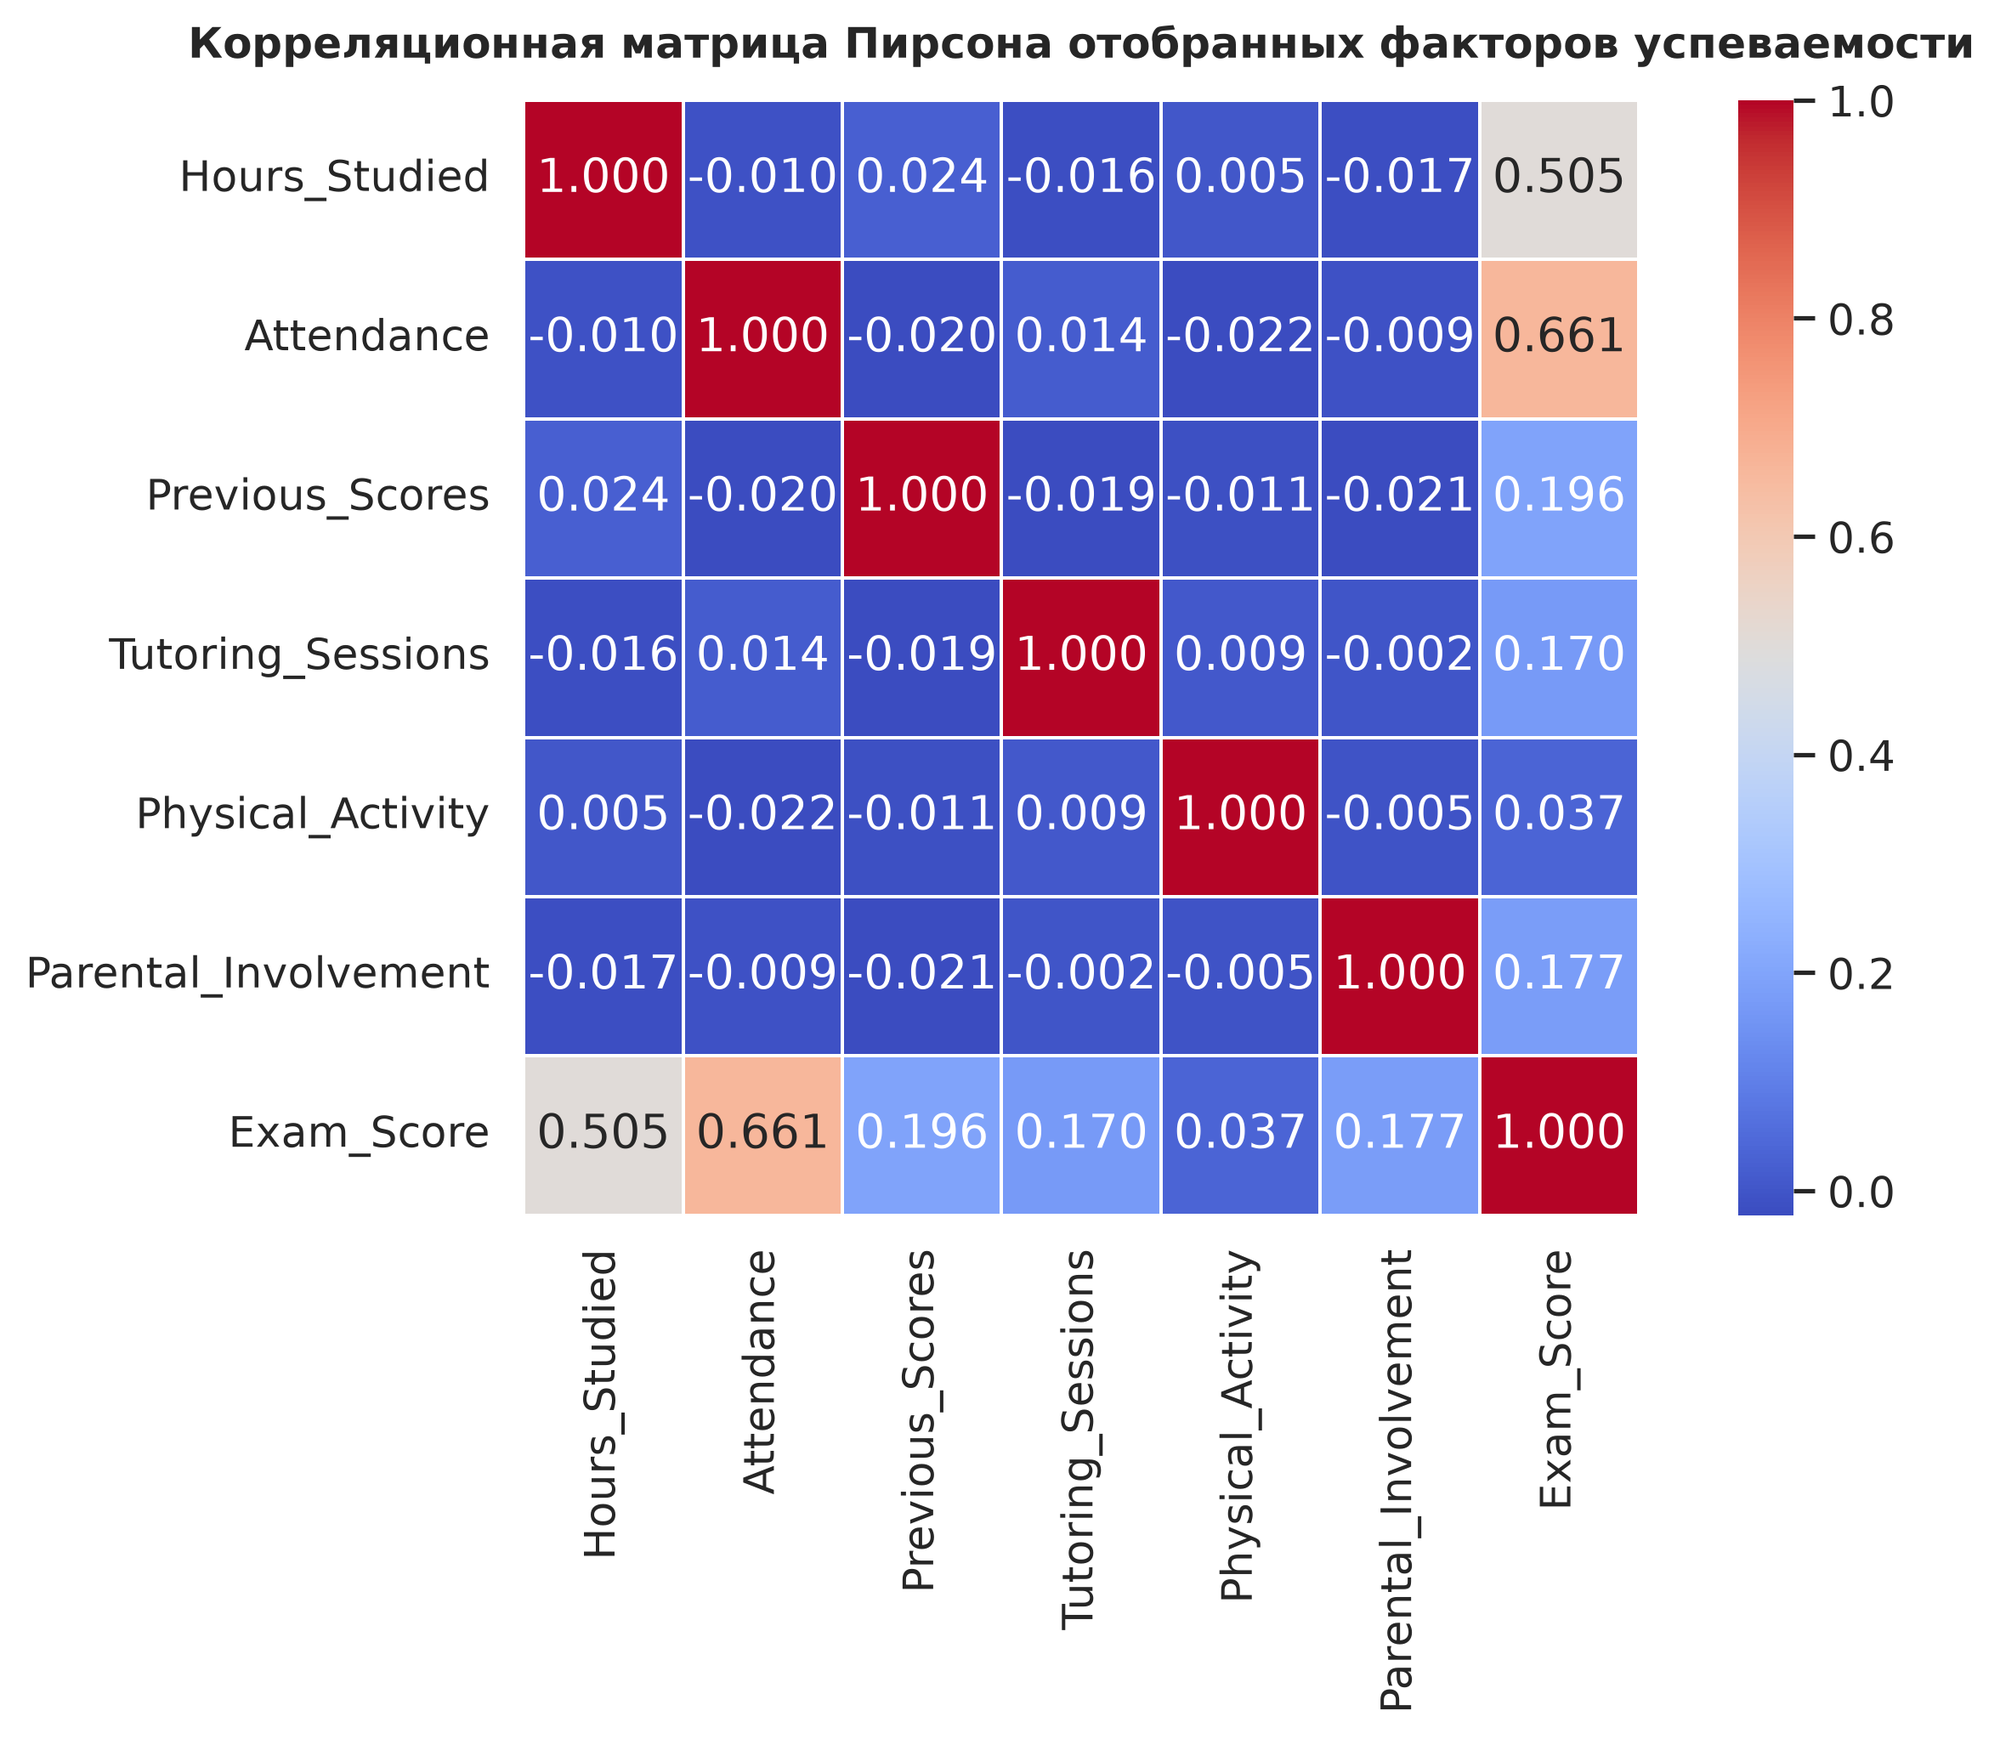
\includegraphics[width=0.88\textwidth]{images/00_correlation_matrix.png}
    \caption{Корреляционная матрица признаков датасета успеваемости студентов}
\end{figure}

На рисунке 2 отображена динамика сходимости MSE при различных значениях шага $\eta \in [0.0005, 0.25]$.

\begin{figure}[H]
    \centering
    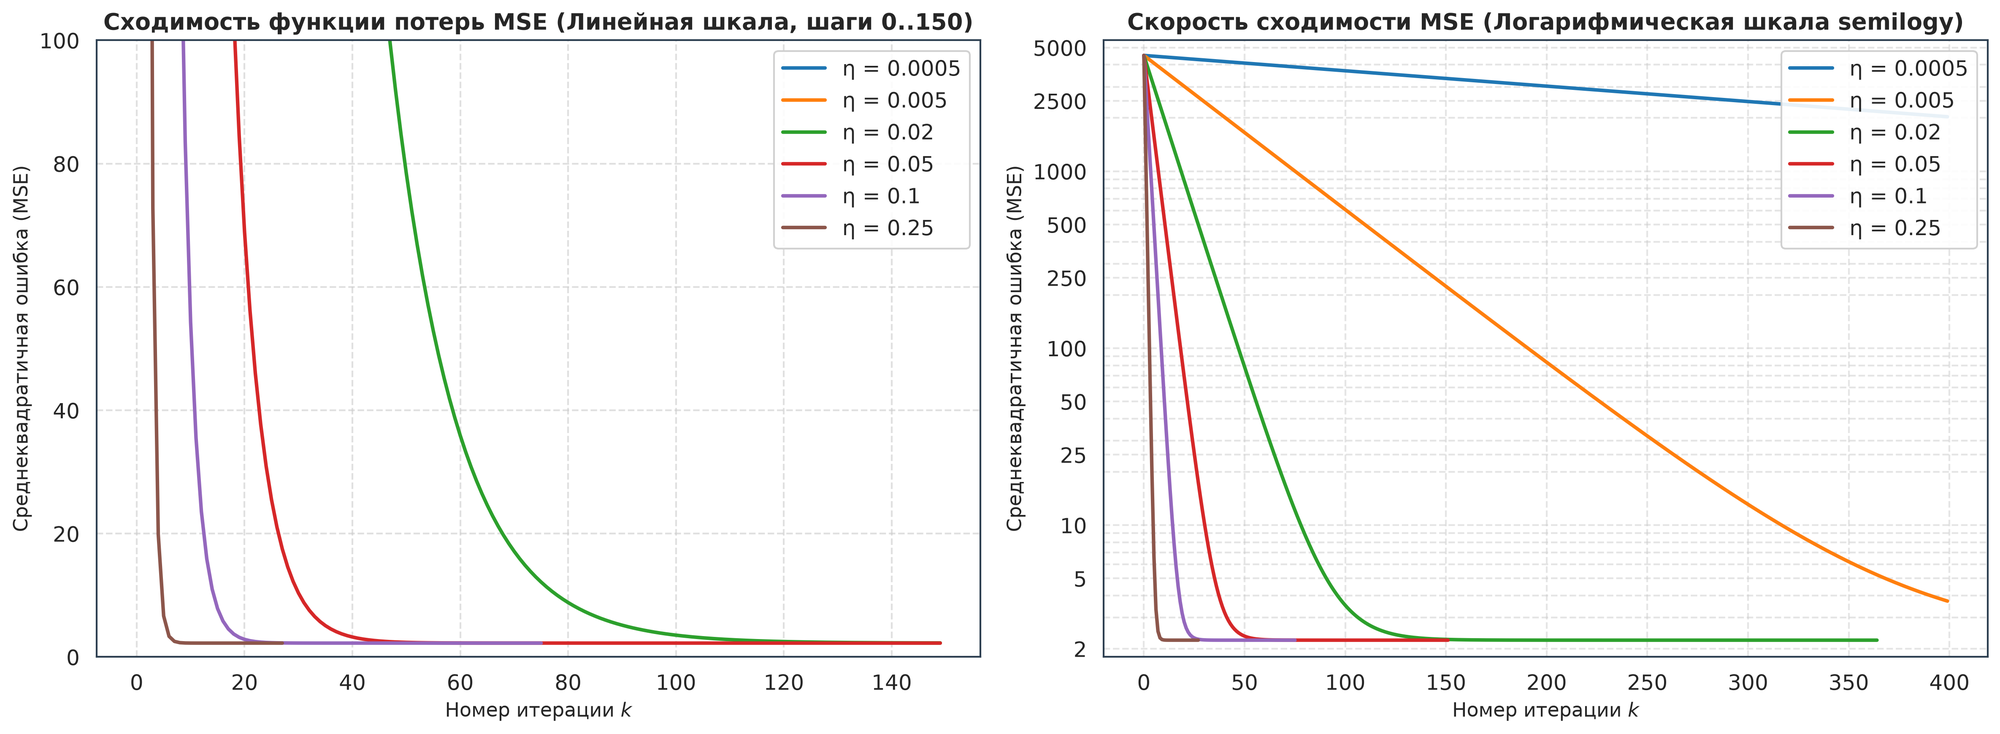
\includegraphics[width=0.92\textwidth]{images/01_learning_rate_experiment.png}
    \caption{Динамика сходимости MSE при различных значениях темпа обучения $\eta$}
\end{figure}

В таблице 1 представлены итоговые характеристики оптимизации при варьировании шага $\eta$.

\begin{table}[H]
\centering
\caption{Влияние темпа обучения $\eta$ на сходимость градиентного спуска}
\begin{tabular}{cccccc}
\toprule
\textbf{Темп $\eta$} & \textbf{Итераций} & \textbf{Сходимость} & \textbf{Test MSE} & \textbf{Test $R^2$} & \textbf{Время (мс)} \\
\midrule
0.0005 & 3000 & Нет (лимит) & 13.4522 & -0.1933 & 813.92 \\
0.0050 & 1337 & Да & 1.9954 & 0.8230 & 366.48 \\
0.0200 & 364 & Да & 1.9954 & 0.8230 & 99.90 \\
0.0500 & 151 & Да & 1.9954 & 0.8230 & 41.44 \\
0.1000 & 75 & Да & 1.9954 & 0.8230 & 21.81 \\
0.2500 & \textbf{27} & \textbf{Да} & \textbf{1.9954} & \textbf{0.8230} & \textbf{8.14} \\
\bottomrule
\end{tabular}
\end{table}

На рисунке 3 продемонстрирована сходимость алгоритмов BGD и SGD на едином графическом поле.

\begin{figure}[H]
    \centering
    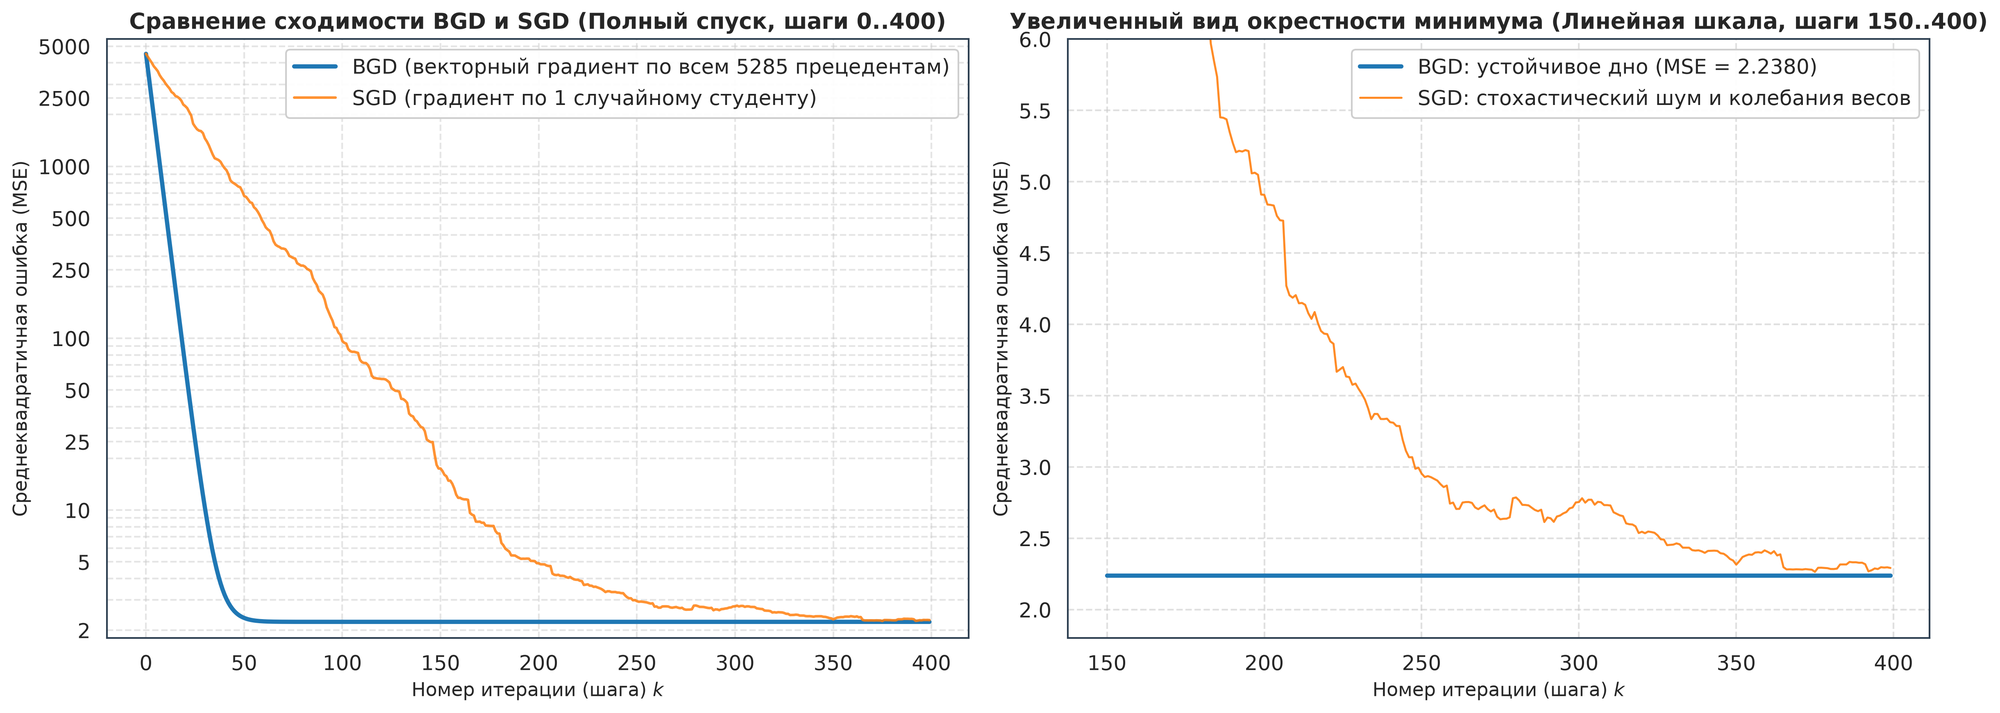
\includegraphics[width=0.92\textwidth]{images/02_gd_vs_sgd_convergence.png}
    \caption{Сравнение сходимости алгоритмов GD и SGD на едином графическом поле}
\end{figure}

В таблице 2 приведены сравнительные вычислительные характеристики алгоритмов.

\begin{table}[H]
\centering
\caption{Сравнительные характеристики пакетного (BGD) и стохастического (SGD) спуска}
\resizebox{\textwidth}{!}{%
\begin{tabular}{lccccc}
\toprule
\textbf{Алгоритм} & \textbf{Размер пакета} & \textbf{Шагов} & \textbf{Test MSE} & \textbf{Test $R^2$} & \textbf{Сложность 1 шага} \\
\midrule
BGD & $l = 5285$ (вся выборка) & 151 & 1.9954 & 0.8230 & $\mathcal{O}(l \cdot m)$ \\
SGD & 1 случайный объект & 10000 & 2.1306 & 0.8110 & $\mathcal{O}(m)$ \\
\bottomrule
\end{tabular}}
\end{table}

На рисунках 4 и 5 представлены регуляризационные пути параметров $w_j$ для 20 значений гиперпараметра $\lambda \in [10^{-3}, 10^3]$ для $L_1$-регуляризации (Lasso) и $L_2$-регуляризации (Ridge).

\begin{figure}[H]
    \centering
    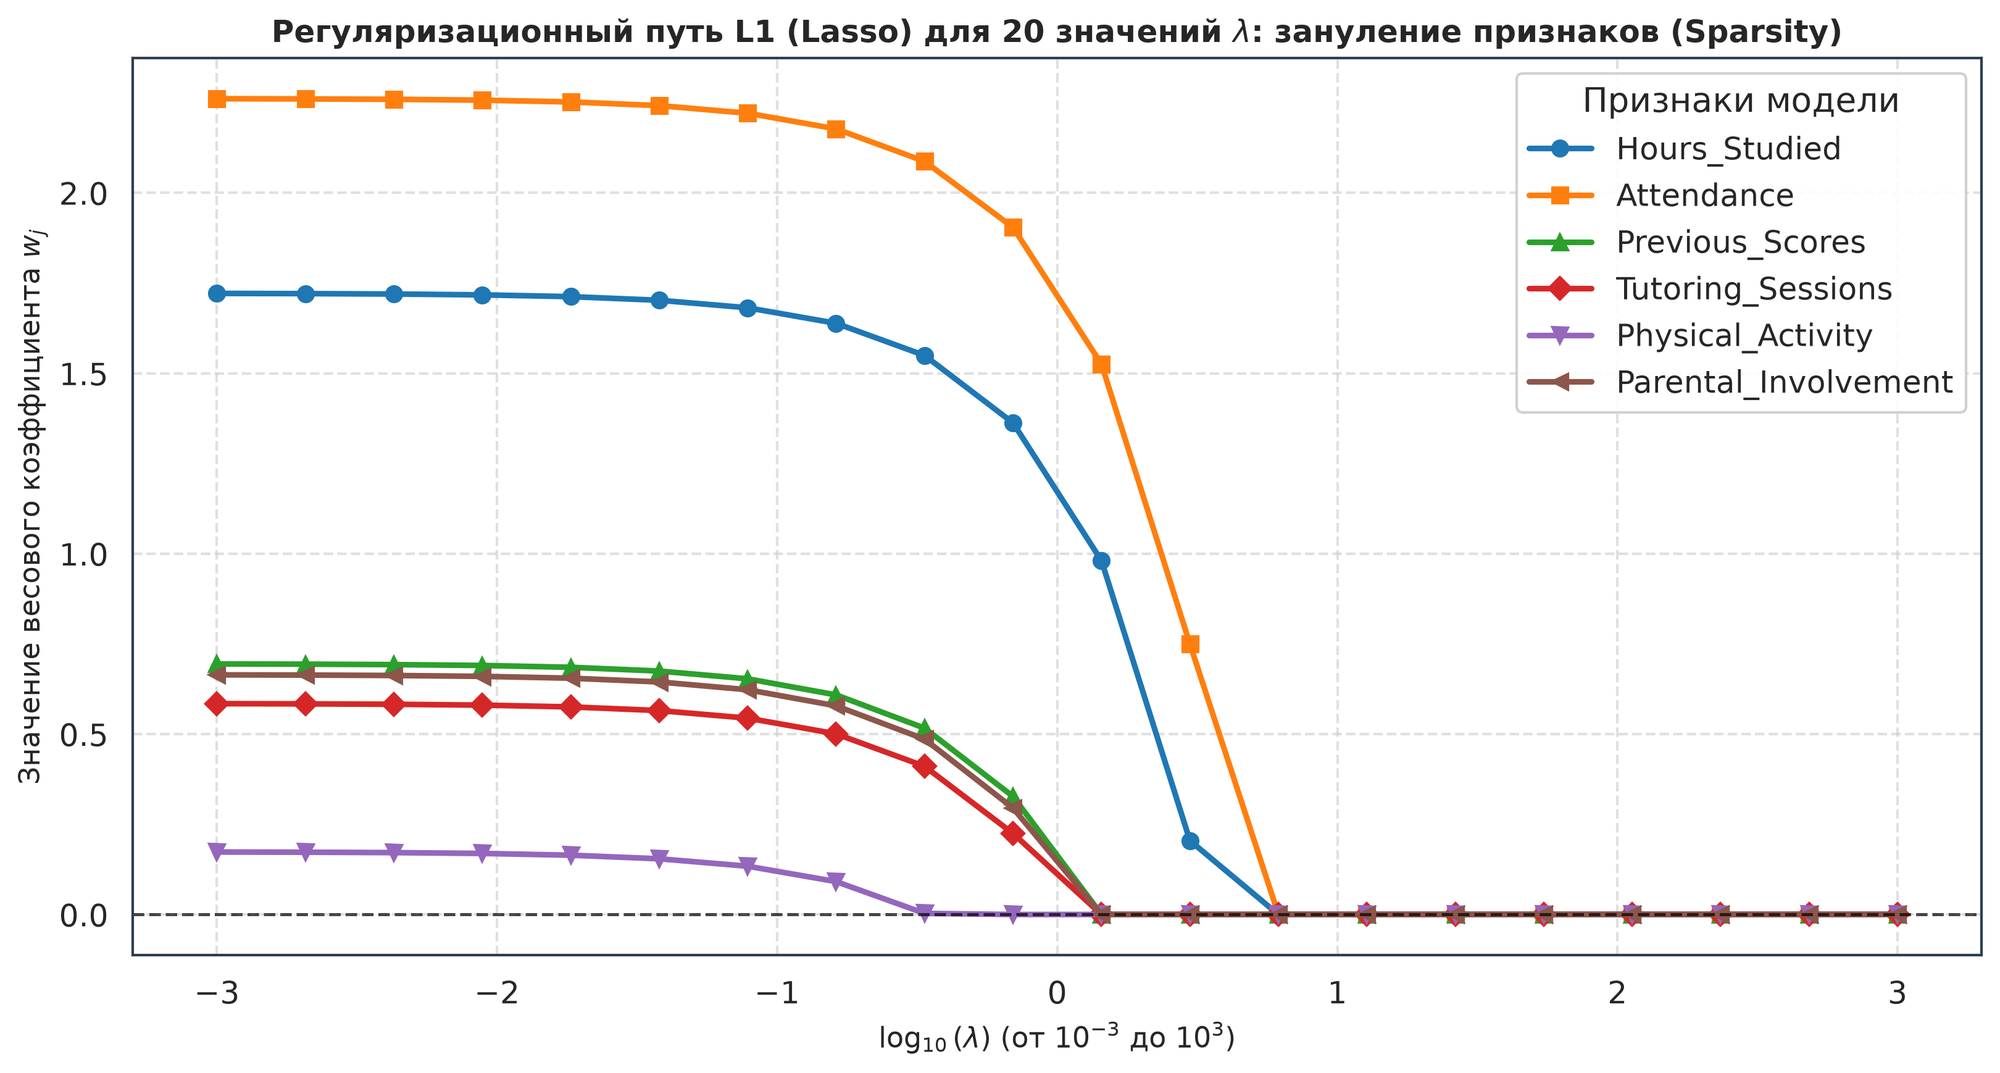
\includegraphics[width=0.90\textwidth]{images/03_l1_regularization_path.png}
    \caption{Регуляризационный путь L1 (Lasso) для варианта 2: зануление признаков (Sparsity)}
\end{figure}

\begin{figure}[H]
    \centering
    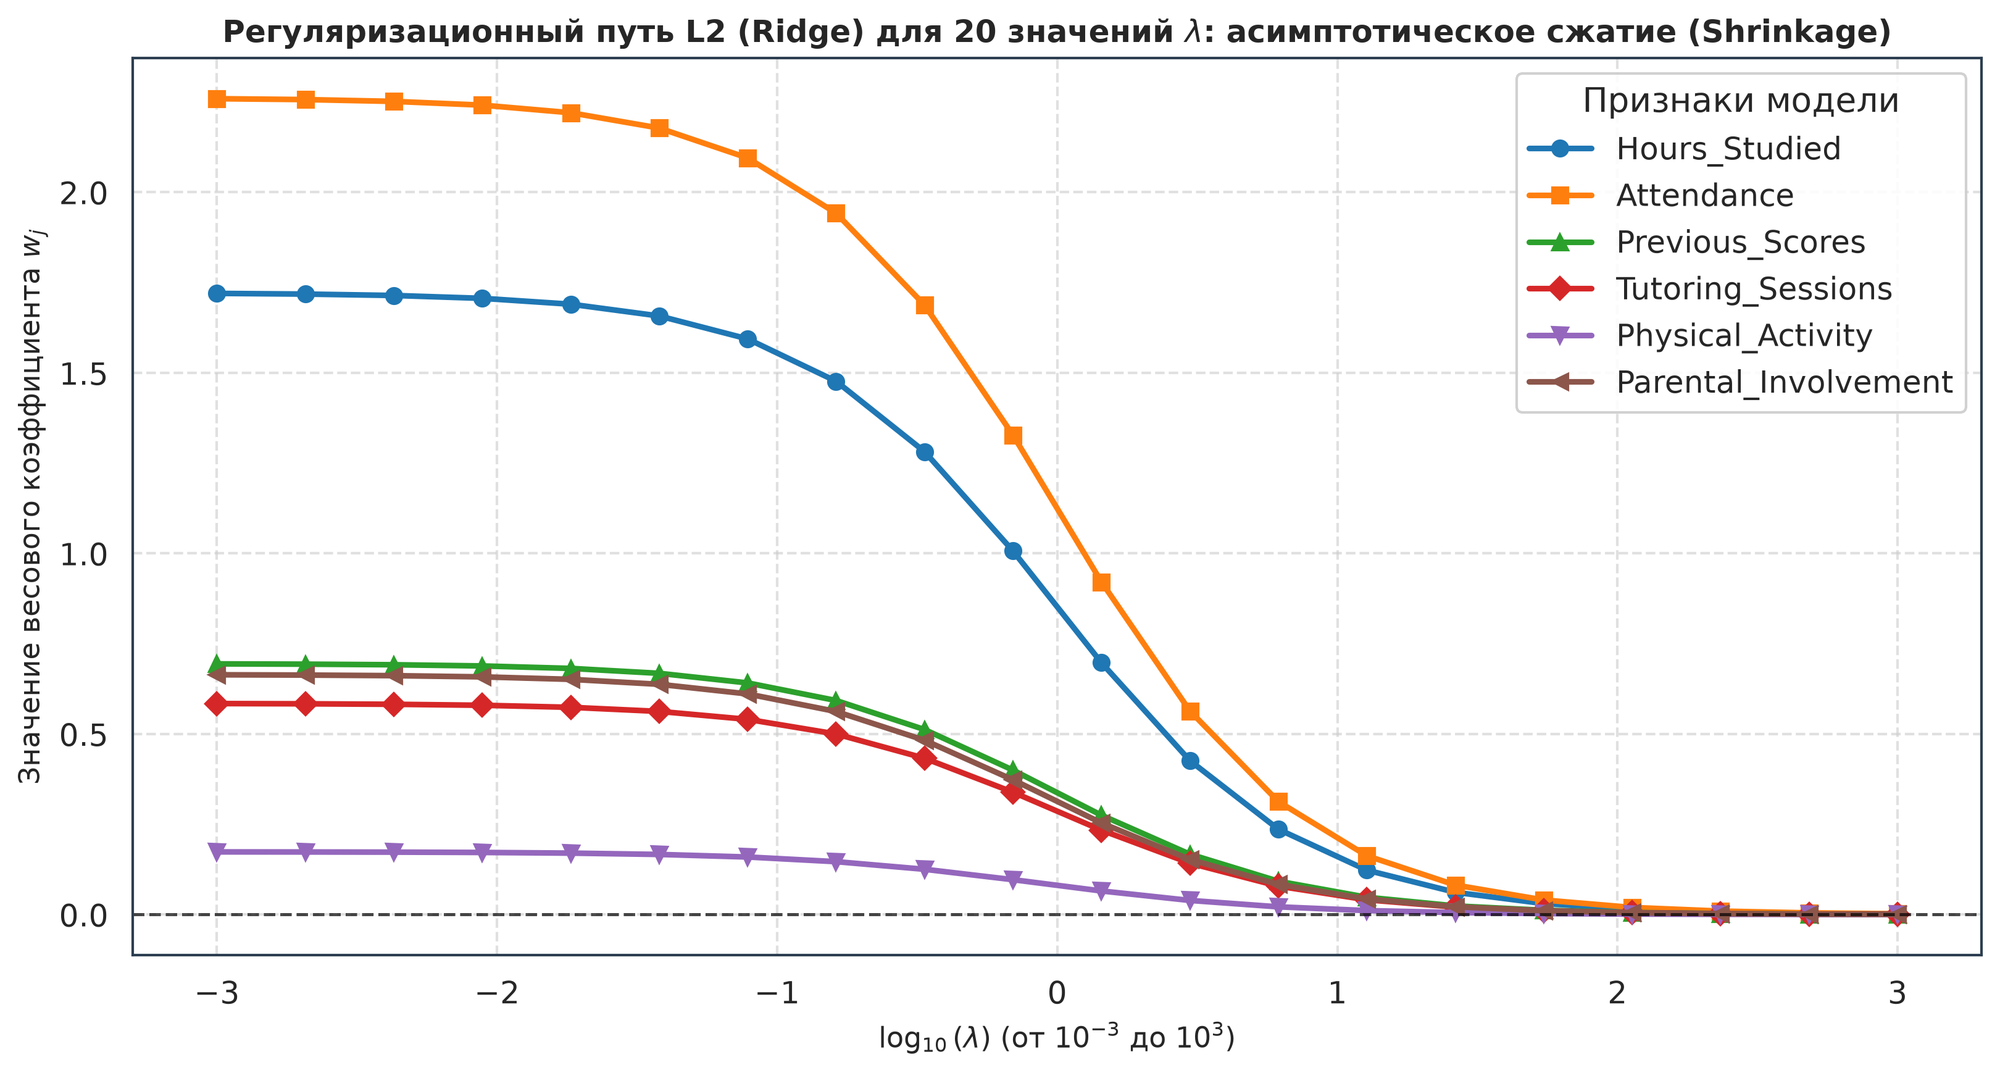
\includegraphics[width=0.90\textwidth]{images/04_l2_regularization_path.png}
    \caption{Регуляризационный путь L2 (Ridge): непрерывное асимптотическое сжатие весов (Shrinkage)}
\end{figure}

На рисунке 6 представлено покомпонентное сопоставление сжатия параметров для каждого фактора модели.

\begin{figure}[H]
    \centering
    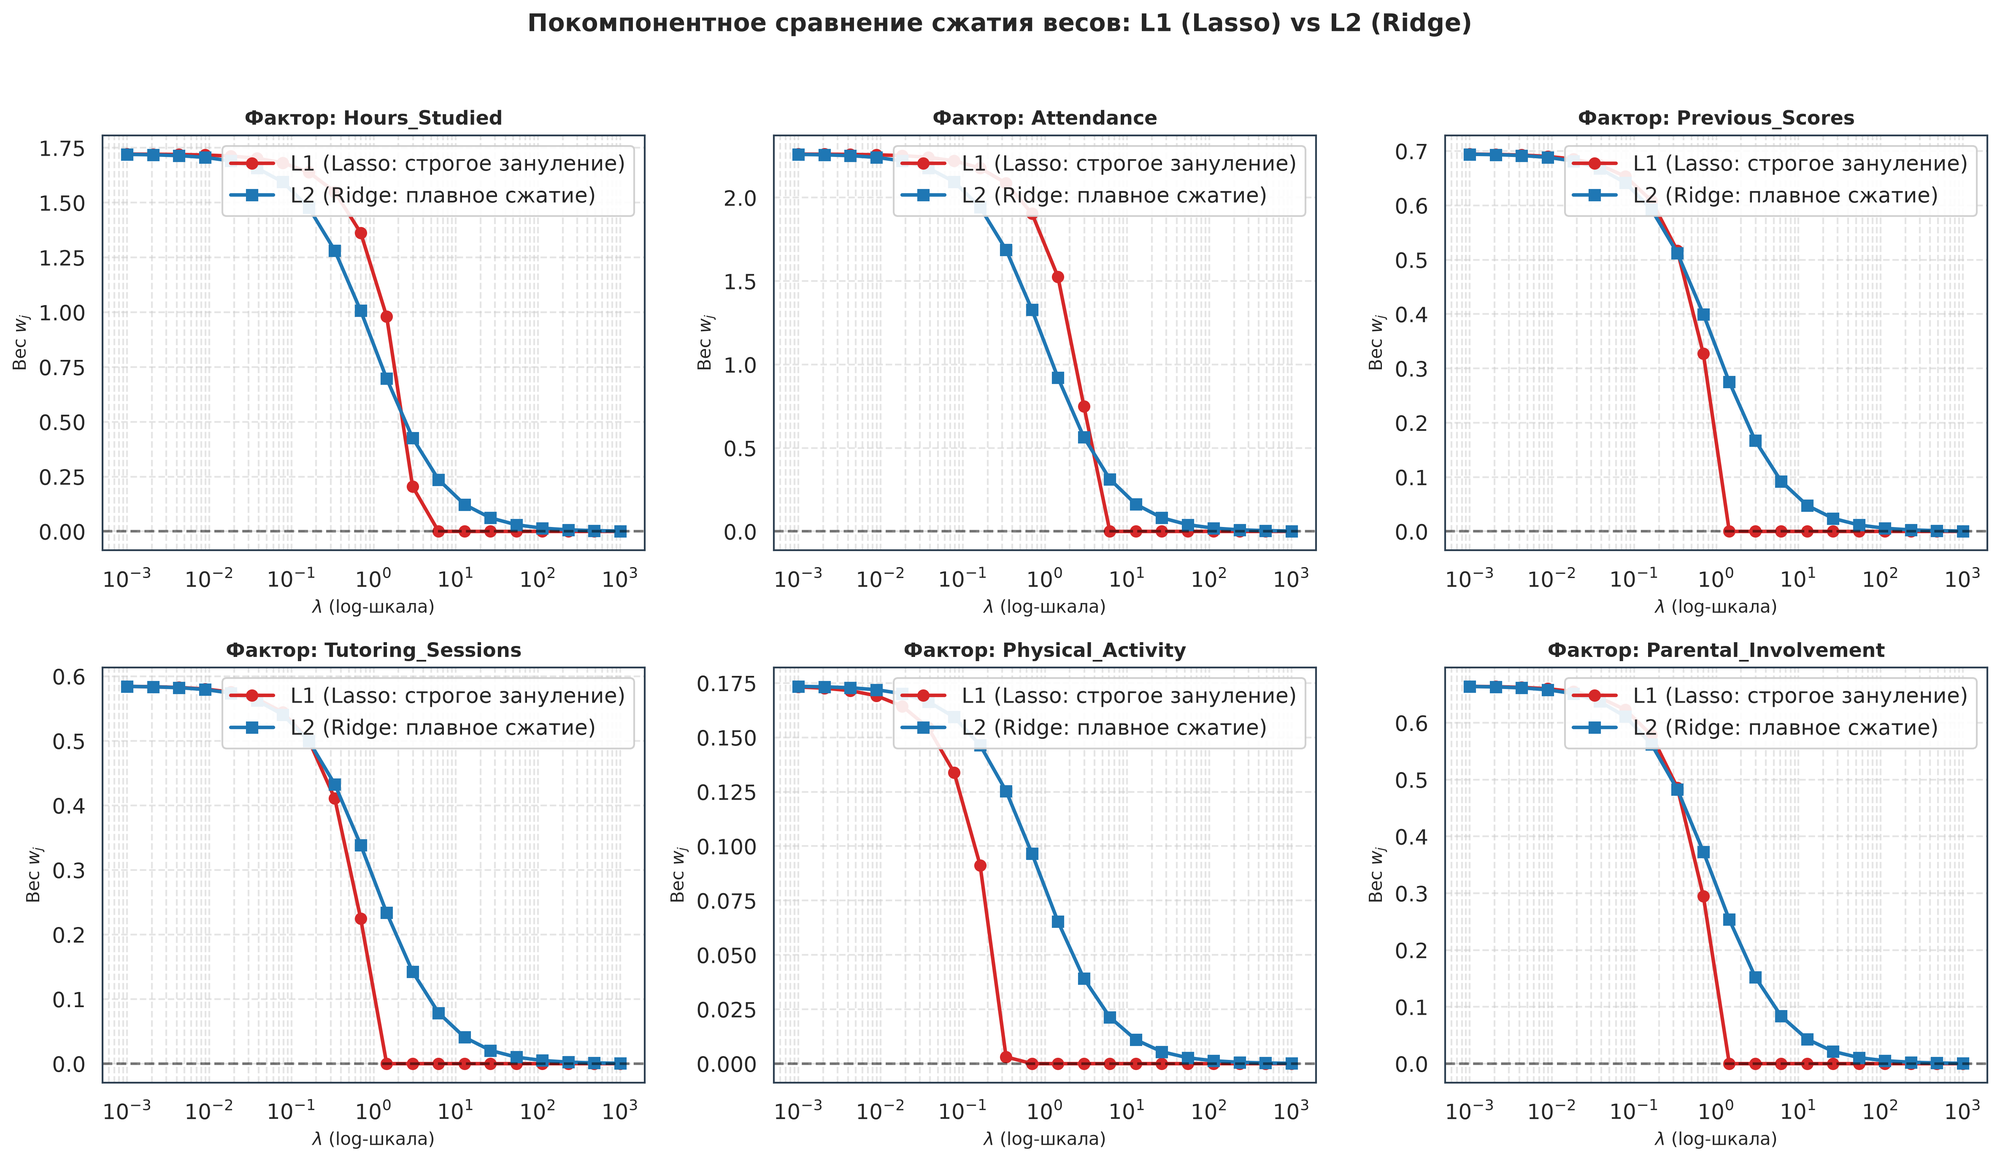
\includegraphics[width=0.95\textwidth]{images/05_regularization_comparison.png}
    \caption{Покомпонентное сравнение отбора признаков (L1) и сжатия коэффициентов (L2)}
\end{figure}

В таблице 3 приведены результаты кросс-валидации собственных алгоритмов против библиотечных эталонов Scikit-Learn.

\begin{table}[H]
\centering
\caption{Результаты эталонного тестирования против библиотеки Scikit-Learn}
\resizebox{\textwidth}{!}{%
\begin{tabular}{lccccc}
\toprule
\textbf{Модель} & \textbf{Intercept $w_0$} & \textbf{$\|w\|_2$} & \textbf{Test MSE} & \textbf{Test MAE} & \textbf{Test $R^2$} \\
\midrule
Custom BGD & 67.0982 & 3.0620 & 1.9954 & 1.0444 & 0.8230 \\
Sklearn OLS & 67.0982 & 3.0620 & 1.9954 & 1.0444 & 0.8230 \\
\midrule
Custom SGD & 67.2268 & 2.8703 & 2.1306 & 1.0951 & 0.8110 \\
Sklearn SGD & 67.1103 & 3.0535 & 1.9923 & 1.0436 & 0.8233 \\
\midrule
Custom L1 ($\lambda=0.5$) & 67.0982 & 2.5707 & 2.3515 & 1.1603 & 0.7914 \\
Sklearn Lasso ($\alpha=0.25$) & 67.0982 & 2.5707 & 2.3515 & 1.1603 & 0.7914 \\
\midrule
Custom L2 ($\lambda=1.0$) & 67.0982 & 1.5129 & 4.3653 & 1.6541 & 0.6128 \\
Sklearn Ridge ($\alpha=5285.0$) & 67.0982 & 1.5129 & 4.3653 & 1.6541 & 0.6128 \\
\bottomrule
\end{tabular}}
\end{table}

На рисунке 7 представлен диагностический дашборд валидации модели: рассеяние предсказаний, распределение остатков и сопоставление весовых параметров.

\begin{figure}[H]
    \centering
    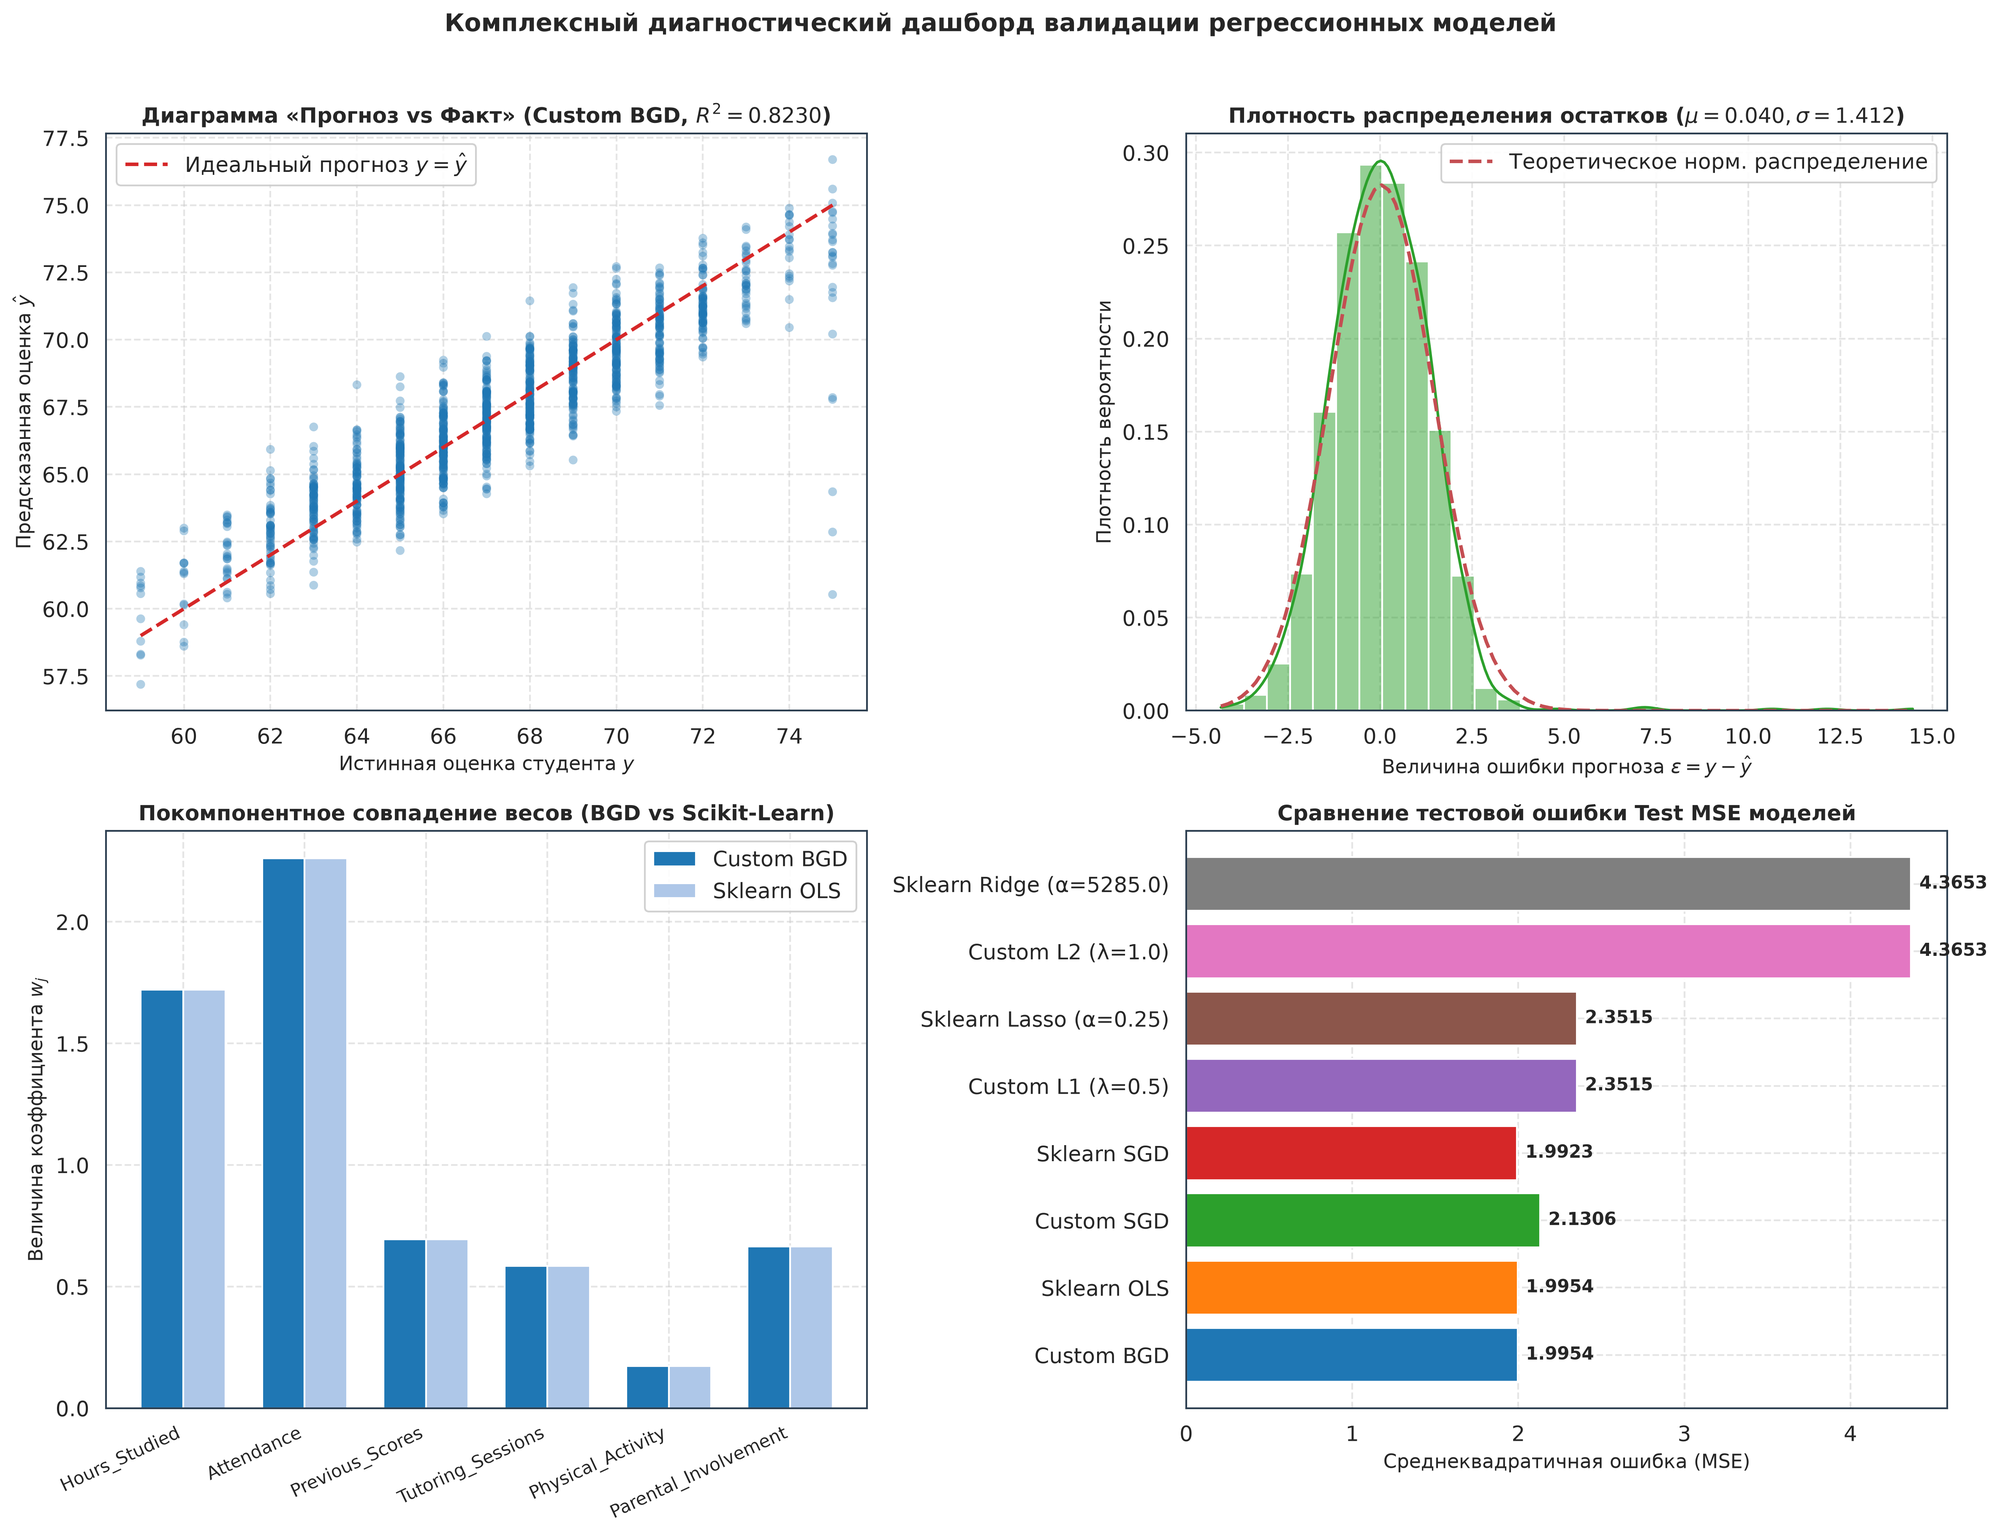
\includegraphics[width=0.95\textwidth]{images/06_model_validation_benchmark.png}
    \caption{Диагностический дашборд валидации модели: рассеяние прогнозов, гистограмма остатков и сопоставление весов}
\end{figure}

% ==============================================================================
% 7. ВЫВОДЫ ПО ЛАБОРАТОРНОЙ РАБОТЕ
% ==============================================================================
\section{Выводы}
\begin{enumerate}
    \item Разработан и верифицирован собственный программный модуль множественной линейной регрессии \texttt{CustomLinearRegression} на чистом векторизованном NumPy. Достигнуто абсолютное численное совпадение найденных весов и метрик качества с библиотечными эталонами Scikit-Learn ($R^2 = 0.8230$, $MSE = 1.9954$).
    \item Экспериментально доказано, что выбор шага обучения $\eta$ играет ключевую роль: при $\eta = 0.25$ алгоритм BGD сошелся за 27 итераций (8.1 мс), тогда как при $\eta = 0.005$ потребовалось 1337 шагов, а при $\eta = 0.0005$ за 3000 шагов оптимум достигнут не был.
    \item Сравнение алгоритмов показало, что пакетный градиентный спуск (BGD) сходится строго монотонно благодаря усреднению градиента по всей выборке ($l = 5285$), а стохастический спуск (SGD) на одном объекте требует на порядок меньше операций на шаг ($\mathcal{O}(m)$ против $\mathcal{O}(lm)$), совершая колебания в окрестности оптимума, стабилизируемые расписанием Роббинса---Монро.
    \item Исследование регуляризационных путей для Варианта 2 наглядно подтвердило фундаментальное теоретическое различие $L_1$ и $L_2$: оператор Soft-Thresholding ($L_1$) обеспечивает зануление весов (Sparsity) и отбор информативных признаков (первым обнуляется \texttt{Physical\_Activity}, последним~--- \texttt{Attendance}), в то время как оператор Weight Decay ($L_2$) непрерывно сжимает все веса к нулю (Shrinkage), сохраняя их ненулевыми.
\end{enumerate}

\end{document}
